\documentclass[11pt]{article}

\usepackage[margin=1.05in]{geometry}
\usepackage{amsmath,amssymb,amsthm}
\usepackage{mathtools}
\usepackage{graphicx}
\usepackage{booktabs}
\usepackage{array}
\usepackage{microtype}
\usepackage{xcolor}
\usepackage[shortlabels]{enumitem}
\usepackage[colorlinks=true,linkcolor=blue!45!black,citecolor=blue!45!black,urlcolor=blue!45!black]{hyperref}
\hypersetup{pdftitle={The middle and the ends I. Uniform Bessel bounds for endpoint crossings in the persistent random walk},pdfauthor={Arjun Pemmasani}}

% ---------- theorem environments ----------
\newtheorem{theorem}{Theorem}[section]
\newtheorem{lemma}[theorem]{Lemma}
\newtheorem{proposition}[theorem]{Proposition}
\newtheorem{corollary}[theorem]{Corollary}
\theoremstyle{definition}
\newtheorem{definition}[theorem]{Definition}
\newtheorem{example}[theorem]{Example}
\theoremstyle{remark}
\newtheorem{remark}[theorem]{Remark}

% ---------- notation macros ----------
\newcommand{\Z}{\mathbb{Z}}
\newcommand{\E}{\mathbb{E}}
\newcommand{\Prob}{\mathbb{P}}
\newcommand{\Var}{\operatorname{Var}}
\newcommand{\Cov}{\operatorname{Cov}}
\newcommand{\chg}{\operatorname{chg}}
\newcommand{\rep}{\operatorname{rep}}
\newcommand{\sL}{\mathsf L}
\newcommand{\sR}{\mathsf R}

\title{The middle and the ends I.\\ Uniform Bessel bounds for endpoint crossings
 in the persistent random walk}
\author{Arjun Pemmasani}
\date{September 26, 2026}
\begin{document}
\maketitle

\begin{abstract}
A persistent random walk takes $N$ steps of $\pm1$, and each step after the
first repeats the one before it with probability $p$. Its steps form the
zero-field Ising chain with free boundaries. Kagey asked when its middle bin
and its endpoints are equally likely. We compare the ratio of each bin to an
endpoint with an explicit Bessel function, with relative error at most
$Nu^2/2+u$ for every bin and every $N$, where $u=(1-p)/p$. At the center this
brackets the crossing $p_N$ for every $N\ge2$. Put $L=\log N$, $T=N(1-p)$ and
$\zeta_N=\frac12W_0(\pi N^2/4)$. The value $z_N$ of $T$ at the crossing lies
below $\zeta_N+1/(8\zeta_N)$ and within $\zeta_N(\zeta_N+1)/N+1/(16\zeta_N^2)$
of it. The proof is analytic for $N\ge175$ and uses exact integer
certificates below that. The whole theorem is also proved in Lean, and the
Lean kernel checks the certificates. As a consequence $z_N$ satisfies the
crossing equation $z_N+\frac12\log z_N=L+c_0+1/(8z_N)+R_N$ with
$c_0=\frac12\log(\pi/8)$ and an explicit bound on $R_N$. We also expand the
crossing of each of the other bins uniformly in its distance from the edge,
with a Laguerre law for fixed bins. Periodic boundaries move the central
crossing by about $(\log2)/N$ in $u$. Finally we prove a local law for the
bin probabilities with a tilted Skellam kernel. Its relative error tends to
$0$ uniformly in $1-p\le\frac12$ away from the edges, from the diffusive to
the ballistic regime.
\end{abstract}

\section{Introduction}\label{sec:intro}

Problem 131 of Kagey's Open Problem Collection~\cite{kagey131} asks about a
Galton board where the ball tends to keep going the same way. The first step
is equally likely to be left or right, and after that each step repeats the
one before it with probability $p$. Kagey asks when the middle bin and the
endpoints are equally likely, and also about his numerator tables, the normal
limit and a board on a cylinder. We answer the main question at every number
of steps, and we treat every interior bin, 2 boundary conditions and the bin
probabilities themselves.

Let $P_N(k)$ be the probability of exactly $k$ right steps in $N$ steps, with
$P_0(0)=1$. Write $q=1-p$, $L=\log N$ and $T=Nq$, and when $p>0$ let $u=q/p$
be the odds of a switch. Only the 2 constant words reach the endpoints, so
$P_N(0)=P_N(N)=\frac12p^{N-1}$ for $N\ge1$. For $N\ge2$ let $p_N$ be the value
of $p$ at which the middle bin and the endpoints are equally likely, which is
unique by Theorem~\ref{thm:root}, and let $z_N=N(1-p_N)$ be the value of $T$
there. Kagey's row $n$ has $N=n-1$, and his numerator tables are in
Remark~\ref{rem:tables}.

The steps of the walk form the zero-field Ising chain with free boundaries.
They are the spins $\sigma_i=\pm1$, a word has weight proportional to
$\exp(J\sum_{i<N}\sigma_i\sigma_{i+1})$ with $e^{-2J}=u$, and the first spin
is uniform. Antal, Droz and R\'acz~\cite{antal2004} give the law of
the magnetization at a fixed scale $T$ under several boundary conditions, and
Dantchev and Rudnick~\cite{dantchev2022} give exact free and periodic
coefficients. The crossing happens when $T$ is of order $\log N$, and there we
need bounds at finite $N$. The Bessel functions in our bounds come from the
confluence of Jacobi, Laguerre and Bessel functions near the point $1$
(Remark~\ref{rem:jacobi}). The zeros of the row polynomial $\sum_kP_N(k)x^k$
are real for $p\le\frac12$, and by the Lee--Yang theorem they lie on the unit
circle for $\frac12\le p<1$ (Remark~\ref{rem:bernoulli}).

\subsection{Results}

Put $S_N(u)=P_N(\lfloor N/2\rfloor)/P_N(0)$, $h=N/2$ and
$F(x)=2x(I_0(2x)+I_1(2x))$. Our first result is the uniform Bessel bound
\[
0\le1-\frac{hS_N(x/h)}{F(x)}\le\frac{x(x+1)}h\qquad(N\ge2,\ x>0)
\]
of Theorem~\ref{thm:bessel}. Theorem~\ref{thm:allbin-bessel} gives the same
kind of bound for every bin, with relative error at most $Nu^2/2+u$. These
bounds hold at every $N$, not only in a limit. At the center they locate the
crossing $p_N$ for every $N$. Let $\zeta_N=\frac12W_0(\pi N^2/4)$ be the positive root
of $8\zeta e^{2\zeta}=\pi N^2$. Theorem~\ref{thm:every-n} says that
\[
\zeta_N+\frac1{8\zeta_N}-\frac{\zeta_N(\zeta_N+1)}N-\frac1{16\zeta_N^2}
<z_N<\zeta_N+\frac1{8\zeta_N}\qquad\text{for every }N\ge2.
\]
The proof is analytic for $N\ge175$. For $2\le N\le174$ it is
computer-assisted, and exact integers decide the sign of $S_N-1$ at 2 points,
one on each side of the root. The whole theorem is also proved in Lean, and
for $N\le174$ the Lean kernel checks these certificates in exact integer
arithmetic. As consequences we get the crossing equation
$z_N+\frac12\log z_N=L+c_0+1/(8z_N)+R_N$ with $c_0=\frac12\log(\pi/8)$ and
$|R_N|\le1/(4L^2)+(L^2+L)/N$ for every $N\ge2$
(Proposition~\ref{prop:crossing-eq}), and the expansion
\[
z_N=L-\tfrac12\log L+c_0+\frac{\frac14\log L-\frac12c_0+\frac18}{L}
+O\Bigl(\frac{(\log L)^2}{L^2}\Bigr)
\]
of Corollary~\ref{cor:every-n}.

For a bin at distance $a$ from the nearer edge,
Theorem~\ref{thm:allbin-expansion} expands the crossing uniformly as
$a\to\infty$, with no condition on how $a$ compares with $N$. For a fixed $a$
the crossing comes instead from a Laguerre polynomial, and the odds $u_{a,b}$
at the crossing have second term $-1/b$ for every fixed bin, where $b=N-a$
(Theorem~\ref{thm:edge-laguerre}). Theorem~\ref{thm:edge-matching} shows that
the 2 regimes match. For odds between the scales $(\log N)/N$ of the central
crossing and $N^{-1/2}$ of the adjacent one, Corollary~\ref{cor:boundary-layer}
gives the width of the layer of bins below the endpoints.

Periodic boundaries move the central crossing in the odds by $(\log2)/N$ to
leading order (Theorem~\ref{thm:periodic-crossing}). Under both boundaries the
ratio of a bin near the center to an endpoint tends to $e^{t-2y^2}$ in the
scaling of Theorem~\ref{thm:critical-window}, and this counts the bins above
the endpoints. Stepanyan et~al.\@~\cite{stepanyan2024} study this periodic
crossing, and Section~\ref{sec:periodicwindow} compares
\eqref{eq:isingtemperature} with their approximations.

Finally, Section~\ref{sec:llt} writes $P_N(k)$ exactly through a difference
of 2 independent binomial variables (Theorem~\ref{thm:llt-identity}) and
approximates it by a tilted symmetric Skellam kernel.
Theorem~\ref{thm:llt} bounds the relative error explicitly for all $0<q<1$,
and by Corollary~\ref{cor:llt} the error tends to $0$ uniformly in
$q\le\frac12$ as the bin moves away from the edges, from the diffusive regime
($q$ fixed) to the ballistic regime ($T$ bounded). The constants are crude.

\subsection{The 4 papers on Problem 131}

\begin{figure}[t]
\centering
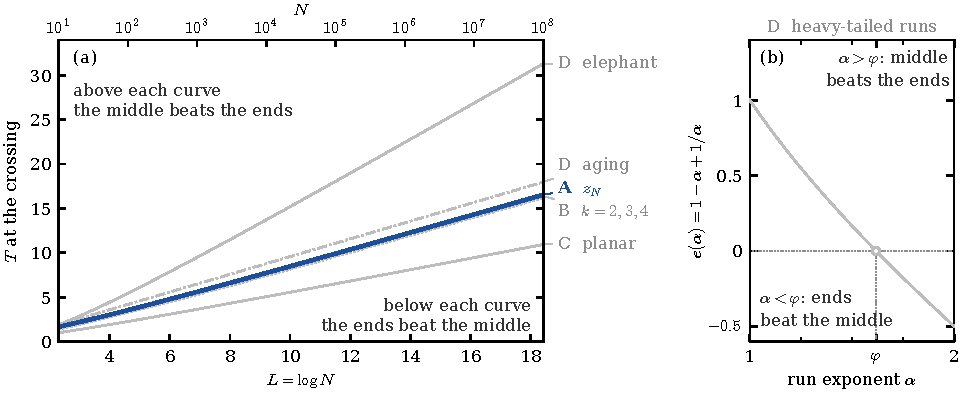
\includegraphics[width=\textwidth]{../figures/program_A}
\caption{(a) The crossing on each model's switching scale against $L=\log N$
for Papers~A to~D. The scale is $T$ for Papers~A to~C, $x=n\varepsilon$ for
the elephant walk and the expected number of switches for the aging walk of
Paper~D. The bold curve is the 2-state crossing $z_N$ of this paper,
and the curves B are the crossings of Paper~B for faces of $k=2,3,4$ states.
(b) The exponent $e(\alpha)=1-\alpha+1/\alpha$ of Paper~D for runs with heavy
tails, which changes sign at the golden ratio $\varphi$.}
\label{fig:program}
\end{figure}

This is the first of 4 papers on Problem 131, and Figure~\ref{fig:program}
shows the crossings of all 4. The present paper treats the walk with 2
states, which is the zero-field one-dimensional Ising chain with free
boundaries. It gives explicit uniform Bessel bounds for every bin and brackets
$p_N$ for every $N\ge2$. The bracket is analytic for $N\ge175$ and rests on
exact certificates below that, and all of it is checked in Lean. The same
bounds give the crossing equation $z_N+\frac12\log z_N=L+c_0+1/(8z_N)+R_N$
with an explicit bound on $R_N$. We also prove a uniform local law for every $q\le\frac12$,
from the diffusive to the ballistic regime. Paper~B~\cite{paperB} treats the
complete graph, a walk on $d$ states that moves to each other state with
probability $T/N$. This is the one-dimensional $d$-state Potts chain. There
every face (set of states) ties with the vertices at first order, and
Paper~B resolves the tie at second order. Its constants $a_k$ are the mass of
a face over a Gaussian volume, square roots of weighted spanning-tree sums,
and the mode changes exactly once, from the vertices to the full centers. A
start law or a weak field shifts the constants. Paper~C~\cite{paperC} gives the general theory for a chain with
transition matrix $P=I+(T/N)Q$ and $T=\tau L$. To first order the mode of the
visit counts sits on a face $F$ that minimizes $\tau\lambda_F+|F|-1$, where
$\lambda_F$ is the principal Dirichlet eigenvalue of $-Q$ on $F$. At second
order a strongly connected face has a constant $K_F$, and the crossings
satisfy a crossing equation. The walks of this paper and of Paper~B are
special cases, and the application is the planar persistent walk.
Paper~D~\cite{paperD} asks what memory changes. The elephant random walk
crosses at $x_n=2z_n-\log(2\pi)+o(1)$ for even $n$, where $z_n$ is the
crossing of this paper at $N=n$. This is about twice the Markov value, and the profile at the
crossing has 2 humps. Runs with heavy tails have a threshold at the golden
ratio, and a short remark treats aging walks. The 4 papers share the notation
$N$, $L$, $T$, $z_N$, $\lambda_F$ and $K_F$.

We prove the exact law in Section~\ref{sec:exact} and the central crossing in
Section~\ref{sec:middle}. Section~\ref{sec:allbin} treats the other bins,
Section~\ref{sec:periodicwindow} periodic boundaries and the window, and
Section~\ref{sec:llt} the local law. Section~\ref{sec:verify} describes the
checks. The longer proofs are in Appendices~\ref{app:every-n}
and~\ref{app:llt}, and Appendix~\ref{app:tables} proves the statements about
Kagey's tables.

\subsection{Related work}

The correlated random walk goes back to Goldstein~\cite{goldstein1951} and
Gillis~\cite{gillis1955}. Renshaw and Henderson~\cite{renshaw1981} study the
same symmetric model, motivated by a Galton machine. They give the exact law
from run counts, the generating function, the normal limit and the upturn at
the endpoints, and in their Section~4 a Bessel limit at a fixed persistence
scale, followed by a limit as that scale grows. Since the 2 limits are taken
one after the other, they give no error bound at finite $N$ when the scale
grows like $\log N$, and the crossing happens at that scale.
Konno~\cite{konno2009} writes the exact law with the hypergeometric function
${}_2F_1$ and proves the telegraph limit when $p=1-\theta/N$ with $\theta$
fixed, which is again a fixed scale, and Herrmann and
Vallois~\cite{herrmann2010} give the telegraph limit with its Bessel density.
Dekking and Kong~\cite{dekkingkong2011} study the Markov binomial law, give its
variance and find when it has 1, 2 or 3 modes. The OEIS
entries~\cite{oeisA035002,oeisA348595} already record both of Kagey's tables.
Stepanyan et~al.\@~\cite[Section~III.B]{stepanyan2024} study the periodic
endpoint--adjacent and endpoint--center crossings directly, so the crossing
question itself is not new. Our bounds hold at finite $N$ when $T$ is of order
$\log N$, also near the edges. The Markov binomial estimates of \v{C}ekanavi\v{c}ius and
Mikalauskas~\cite{cekanavicius2001,cekanavicius2001ld} assume ranges of the
transition probabilities that exclude $p\to1$. Section~\ref{sec:llt} discusses
the work on local limits.

\section{The exact law}\label{sec:exact}

The results of this section are classical~\cite{renshaw1981,dekkingkong2011}.
We prove Theorem~\ref{thm:pmf} because the later sections use its count of
words by switches. By \eqref{eq:wordprob}, a word with $j$ switches has
probability $\frac12p^{N-1-j}q^j$.

\begin{theorem}[bin probabilities]\label{thm:pmf}
Let $N\ge1$. Then $P_N(0)=P_N(N)=\tfrac12p^{N-1}$, and for $1\le k\le N-1$
\[
P_N(k)=\frac12\sum_{j=1}^{N-1}W(N,k,j)\,p^{N-1-j}q^{\,j},
\]
where, writing $a=k$ and $b=N-k$,
\[
W(N,k,2i-1)=2\binom{a-1}{i-1}\binom{b-1}{i-1},\qquad
W(N,k,2i)=\binom{a-1}{i}\binom{b-1}{i-1}+\binom{a-1}{i-1}\binom{b-1}{i}
\]
is the number of words with $a$ letters $\sR$, $b$ letters $\sL$ and exactly
$j$ switches.
\end{theorem}

\begin{proof}
By \eqref{eq:wordprob} it suffices to count the words in bin $k$ with $j$
switches. We count them by their run lengths. A word with $j$ switches
consists of $j+1$ maximal runs, alternately of letters $\sR$ and of letters
$\sL$. If $k\in\{0,N\}$ there is one word and it has no switch. Let $a,b\ge1$.
If $j+1=2i$ there are $i$ runs of each letter. The run lengths form a
composition of $a$ into $i$ parts and a composition of $b$ into $i$ parts, and
there are $\binom{a-1}{i-1}\binom{b-1}{i-1}$ such pairs. The two choices of the
first letter give the factor $2$. If
$j+1=2i+1$ the word starts and ends with the same letter. Starting with $\sR$
gives $i+1$ runs of $\sR$ and $i$ runs of $\sL$, so
$\binom{a-1}{i}\binom{b-1}{i-1}$ words, and starting with $\sL$ gives the
other summand.
\end{proof}

For instance $P_2=(\tfrac p2,\,q,\,\tfrac p2)$, $P_3(1)=\tfrac12(1-p^2)$ and
$P_4(2)=q(1-p+p^2)$. Each interior bin needs at least one switch, while the
endpoints need none. So the endpoints win when $p$ is close to $1$, and
Section~\ref{sec:middle} asks how close.

\begin{proposition}[recurrence and generating function]\label{prop:gf}
Let $P_N^{\sR}(k)$ and $P_N^{\sL}(k)$ be the probabilities of being in bin $k$
after $N$ steps with last letter $\sR$, respectively $\sL$, and set them to $0$
outside $0\le k\le N$. Then $P_1^{\sR}(1)=P_1^{\sL}(0)=\tfrac12$,
$P_1^{\sR}(0)=P_1^{\sL}(1)=0$, and for $N\ge2$
\begin{equation}\label{eq:dp}
P_N^{\sR}(k)=p\,P_{N-1}^{\sR}(k-1)+q\,P_{N-1}^{\sL}(k-1),\qquad
P_N^{\sL}(k)=p\,P_{N-1}^{\sL}(k)+q\,P_{N-1}^{\sR}(k).
\end{equation}
Consequently
\begin{equation}\label{eq:gf}
\sum_{N\ge0}\sum_{k=0}^{N}P_N(k)\,x^kt^N=\frac{1-(p-\tfrac12)(1+x)\,t}{1-p(1+x)\,t+(2p-1)\,x\,t^2},
\end{equation}
and for all $N\ge2$ and all $k$, with $P_M(k)=0$ outside $0\le k\le M$,
\begin{equation}\label{eq:rec}
P_N(k)=p\bigl(P_{N-1}(k)+P_{N-1}(k-1)\bigr)-(2p-1)\,P_{N-2}(k-1).
\end{equation}
\end{proposition}

\begin{proof}
The recursion \eqref{eq:dp} follows by conditioning on $w_{N-1}$, since $w_N$
equals $w_{N-1}$ with probability $p$.
Let $H^{\sR}=\sum_{N,k}P_N^{\sR}(k)x^kt^N$ and define $H^{\sL}$ alike. By
\eqref{eq:dp}, $H^{\sR}=xt(\tfrac12+pH^{\sR}+qH^{\sL})$ and
$H^{\sL}=t(\tfrac12+pH^{\sL}+qH^{\sR})$. Solving these two linear equations
and adding $1$ for $N=0$ gives \eqref{eq:gf}, which is the generating function
of Renshaw and Henderson~\cite{renshaw1981} in our notation. Multiplying
\eqref{eq:gf} by its denominator and comparing the coefficients of $x^kt^N$
with $N\ge2$ gives \eqref{eq:rec}.
\end{proof}

\begin{remark}[numerator tables]\label{rem:tables}
For $p=\alpha/(\alpha+\beta)$ with integers $\alpha,\beta\ge0$, not both $0$,
the numerators of the tables of the problem are
$n_N(k)=2(\alpha+\beta)^{N-1}P_N(k)$ for $N\ge1$, not reduced. By
\eqref{eq:wordprob}, $n_N(k)$ is the sum of $\alpha^{\rep(w)}\beta^{\chg(w)}$
over the words with $k$ letters $\sR$ and $N-k$ letters $\sL$, which shows that
it is an integer.
\end{remark}

\subsection{Variance and the normal limit}\label{sec:clt}

Note that $K_N$ counts the visits of the chain $w_1,\dots,w_N$ to the letter
$\sR$. This chain leaves each letter with probability $q$ and starts from its
stationary law $(\frac12,\frac12)$. So $K_N$ has the Markov binomial law
$\mathrm{Bin}(N,q,q,(\frac12,\frac12))$ of Dekking and
Kong~\cite{dekkingkong2011}, whose second eigenvalue is $1-2q=2p-1$.

\begin{proposition}[mean and variance]\label{prop:var}
Let $0<p<1$ and $\rho=2p-1$. Then $\E K_N=N/2$ and
\[
\Var K_N=\frac14\Bigl(N\,\frac{1+\rho}{1-\rho}-\frac{2\rho\,(1-\rho^N)}{(1-\rho)^2}\Bigr)
=\frac{Np}{4(1-p)}-\frac{(2p-1)\bigl(1-(2p-1)^N\bigr)}{8(1-p)^2}.
\]
\end{proposition}

\begin{proof}
This is \cite[Eq.~(2.3) and Proposition~2.1]{dekkingkong2011} with $a=b=q$
and the stationary start, for which both excentricities vanish and both
stationary weights are $\frac12$. The second form follows from
$(1+\rho)/(1-\rho)=p/q$ and $1-\rho=2q$.
\end{proof}

\begin{theorem}[normal limit]\label{thm:clt}
Let $0<p<1$ be fixed. Then $(K_N-N/2)/\sqrt N$ converges in distribution, as
$N\to\infty$, to the normal law with mean $0$ and variance $p/(4(1-p))$.
\end{theorem}

So persistence keeps the bell shape but widens it by the factor $\sqrt{p/q}$
compared with the ordinary board.

\begin{proof}
Let $v_N(\theta)$ be the vector with entries
$\E[e^{i\theta X_N};\sigma_N=\pm1]$. By \eqref{eq:dp}, $v_{N+1}=Mv_N$ with
\[
M=\begin{pmatrix}pe^{i\theta}&qe^{i\theta}\\qe^{-i\theta}&pe^{-i\theta}\end{pmatrix},\qquad
\operatorname{tr}M=2p\cos\theta,\quad\det M=2p-1 .
\]
At $\theta=0$ the eigenvalues are $1$ and $2p-1$, which are distinct. So for
small $|\theta|$ the matrix $M$ has the simple eigenvalue
$\lambda_+(\theta)=p\cos\theta+\sqrt{q^2-p^2\sin^2\theta}
=1-\frac p{2q}\theta^2+O(\theta^4)$ and the other eigenvalue stays near $2p-1$,
with spectral projections $\Pi_\pm(\theta)$ that depend continuously on
$\theta$, because the two eigenvalues are simple. Write $\mathbf 1=(1,1)$. Then
$\E e^{i\theta X_N}=\mathbf 1\cdot M^{N-1}v_1(\theta)
=\lambda_+^{N-1}\,\mathbf 1\cdot\Pi_+v_1+\lambda_-^{N-1}\,\mathbf 1\cdot\Pi_-v_1$.
The vector $v_1(0)=(\frac12,\frac12)$ is an eigenvector of $M$ for the
eigenvalue $1$ at $\theta=0$, so $\mathbf 1\cdot\Pi_+v_1\to1$ as $\theta\to0$,
while $|\lambda_-|\to|2p-1|<1$. Put $\theta=s/\sqrt N$ with $s$ fixed. Then
the second term tends to $0$, and the first tends to $\exp(-\frac p{2q}s^2)$
since $(N-1)\log\lambda_+(s/\sqrt N)\to-\frac p{2q}s^2$. By
L\'evy's continuity theorem
\cite[Theorem~26.3]{billingsley1995}, $X_N/\sqrt N$ converges to the normal
law with variance $p/q$. Finally $K_N-N/2=X_N/2$.
\end{proof}

\section{The central crossing at every \texorpdfstring{$N$}{N}}\label{sec:middle}

Let $N\ge2$, let $m_N=\lfloor N/2\rfloor$
and let $p>0$. By Theorem~\ref{thm:pmf} the ratio of the middle bin to an
endpoint is
\begin{equation}\label{eq:SN}
\frac{P_N(m_N)}{P_N(0)}=S_N(u):=\sum_{j=1}^{N-1}W(N,m_N,j)\,u^j ,
\end{equation}
a polynomial in $u$ with nonnegative integer coefficients and
$W(N,m_N,1)=2$. The middle and the endpoints are level exactly when
$S_N(u)=1$.

The following heuristic explains why this happens when $T$ is near $\log N$.
Let $a=m_N$ and
$b=N-m_N$, both about $N/2$. A word in the middle bin with $2r+1$ switches has
$r+1$ runs of each letter, and there are
$2\binom{a-1}r\binom{b-1}r\approx2(N/2)^{2r}/(r!)^2$ of them when $r$ is small
compared with $\sqrt N$. So these words contribute about
$2u\sum_r(Nu/2)^{2r}/(r!)^2=2uI_0(Nu)$ to $S_N(u)$, and in the same way the
words with an even number of switches contribute about $2uI_1(Nu)$. For large
$w=Nu$ we have $I_0(w)+I_1(w)\approx2e^w/\sqrt{2\pi w}$, so
$S_N(u)\approx4we^w/(N\sqrt{2\pi w})$. Setting this equal to $1$ gives
$w+\frac12\log w\approx L+\frac12\log(\pi/8)$. So at the crossing $w$, and with
it $T$, is close to $L-\frac12\log L+c_0$ with $c_0=\frac12\log(\pi/8)$.

\begin{theorem}\label{thm:root}
\begin{enumerate}[(a)]
\item For every $N\ge2$ there is exactly one $p=p_N\in[0,1]$ with
$P_N(m_N)=P_N(0)$, and $p_N\ge\tfrac23$. The middle is more likely than the
endpoints for $p<p_N$ and less likely for $p>p_N$.
\item $p_2=\tfrac23$, $p_3=1/\sqrt2$, $p_4$ is the real root of
$3p^3-4p^2+4p-2$, and $p_N<p_{N+1}$ for all $N\ge2$.
\item $p_N\to1$ as $N\to\infty$, and more precisely $1-p_N\sim(\log N)/N$.
\end{enumerate}
\end{theorem}

\begin{proof}
(a) At $p=0$ the endpoints have probability $0$ and the middle does not. For
$p>0$ the equation is $S_N(u)=1$ by \eqref{eq:SN}. The coefficients of $S_N$
are nonnegative and the linear one is $2$, so $S_N$ is strictly increasing on
$[0,\infty)$ with $S_N(0)=0$ and $S_N(u)\ge2u$. By the intermediate value
theorem there is exactly one root $u_N\in(0,\tfrac12]$. The map
$u\mapsto p=1/(1+u)$ is a decreasing bijection from $[0,\infty)$ to $(0,1]$.
Hence $p_N=1/(1+u_N)\ge\tfrac23$, and the middle wins exactly when $u>u_N$.

(b) By Theorem~\ref{thm:pmf}, $S_2=2u$, $S_3=2u+u^2$ and $S_4=2u+2u^2+2u^3$,
which give the three values. For $p_4$,
substitute $u=(1-p)/p$ in $S_4(u)=1$. For the monotonicity we compare
coefficients. Going from $N$ to $N+1$, one entry of the middle pair
$(a,b)=(\lfloor N/2\rfloor,\lceil N/2\rceil)$ grows by one and the other is
unchanged. The formulas of Theorem~\ref{thm:pmf} are symmetric in $(a,b)$, and
every $\binom{a-1}{\cdot}$ is nondecreasing in $a$. So
$W(N+1,m_{N+1},j)\ge W(N,m_N,j)$ for every $j$. The coefficient of $u^2$ is
$a+b-2=N-2$, which increases strictly. Hence $S_{N+1}(u)>S_N(u)$ for $u>0$, so
$u_{N+1}<u_N$.

(c) We prove (c) after Theorem~\ref{thm:bessel}, from part~(i) of that
theorem.
\end{proof}

In the tables of the problem, the middle and the endpoints of row $N+1$ are
level at $p=p_N$. The least value is $p_2=\tfrac23$ for the odd rows and
$p_3=1/\sqrt2$ for the even rows after the second (which is $1,1$ for every
$p$). There is no greatest value, since $p_N\uparrow1$. The tenth row has $p_9=0.82829\ldots$, just below
$\tfrac56$, so its middle and endpoints are nearly level in the third histogram of the
problem
(Figure~\ref{fig:row10} and Table~\ref{tab:pn}).

\begin{figure}[t]
\centering
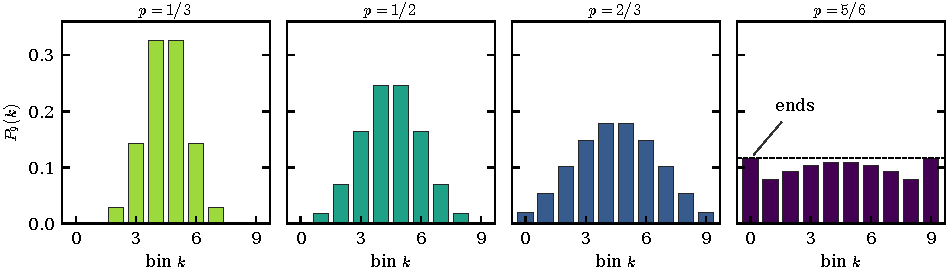
\includegraphics{figures/row10}
\caption{The bin probabilities $P_9(k)$ of the tenth row for
$p=\frac13,\frac12,\frac23,\frac56$. At $p=\frac56$, just above $p_9$, the two middle bins are
slightly below the endpoints (dashed line).}
\label{fig:row10}
\end{figure}

\begin{table}[ht]
\centering\small
\begin{tabular}{@{}rl@{\hskip 2em}rl@{\hskip 2em}rl@{\hskip 2em}rl@{}}
\toprule
$N$ & $p_N$ & $N$ & $p_N$ & $N$ & $p_N$ & $N$ & $p_N$\\
\midrule
2 & 0.66666667 & 6 & 0.78871211 & 10 & 0.83840411 & 50 & 0.94200405\\
3 & 0.70710678 & 7 & 0.80361731 & 11 & 0.84652725 & 100 & 0.96496633\\
4 & 0.74487450 & 8 & 0.81759938 & 12 & 0.85426060 & 200 & 0.97939018\\
5 & 0.76759188 & 9 & 0.82829163 & 20 & 0.89293837 & 400 & 0.98812464\\
\bottomrule
\end{tabular}
\caption{The value $p_N$ at which the middle and endpoint bins of row $N+1$ are equally likely.}
\label{tab:pn}
\end{table}

\subsection{A Bessel bound at every \texorpdfstring{$N$}{N}}

The heuristic above replaced the number $\binom{a-1}{r}$ of ways to split $a$
letters into $r+1$ runs by $a^r/r!$. After this change the run count is
exactly the power series of $I_0$ and $I_1$. The next lemma controls the error
of this change.

\begin{lemma}[clipped products]\label{lem:clipped}
(a) If $t_1,\dots,t_r\ge0$ and $(v)_+=\max(v,0)$, then
$0\le1-\prod_{k=1}^r(1-t_k)_+\le\sum_{k=1}^rt_k$.
(b) For integers $m\ge1$ and $r\ge0$,
$U_r(m):=\frac{r!}{m^r}\binom{m-1}{r}=\prod_{k=1}^r\bigl(1-\frac km\bigr)_+$,
so $0\le1-U_r(m)\le\frac{r(r+1)}{2m}$.
(c) For $x\ge0$,
\begin{gather*}
\sum_{r\ge0}\frac{r(r+1)x^{2r}}{(r!)^2}=x^2I_0(2x)+xI_1(2x),\\
\sum_{r\ge0}\frac{r(r+1)x^{2r+1}}{r!(r+1)!}=x^2I_1(2x),\qquad
\sum_{r\ge0}\frac{(r+1)x^{2r+1}}{r!(r+1)!}=xI_0(2x).
\end{gather*}
\end{lemma}

\begin{proof}
(a) Every factor lies in $[0,1]$, so the product is at most $1$. If some
$t_k\ge1$ the product is $0$ and the sum is at least $1$. Otherwise
$\prod_k(1-t_k)\ge1-\sum_kt_k$ by induction on $r$. (b) Note that
$\frac{r!}{m^r}\binom{m-1}{r}=\prod_{k=1}^r\frac{m-k}m$. For $r<m$ every factor
is positive, and for $r\ge m$ both sides vanish, the right side through the
factor $k=m$. The bound is (a) with $t_k=k/m$. (c) Use the series of $I_0(2x)$
and $I_1(2x)$ from Section~\ref{sec:setting}. Write $r(r+1)=r^2+r$ in the
first sum, cancel the factors $r$ and $r+1$ against the factorials, and shift
the index.
\end{proof}

\begin{theorem}[uniform Bessel approximation]\label{thm:bessel}
Put $h=N/2$ and $F(x)=2x\bigl(I_0(2x)+I_1(2x)\bigr)$, and recall that
$u_N=(1-p_N)/p_N$.
\begin{enumerate}[(i)]
\item For every $N\ge2$ and $x>0$,
\begin{equation}\label{eq:uniformbessel}
0\le1-\frac{hS_N(x/h)}{F(x)}\le\frac{x(x+1)}h.
\end{equation}
\item Let $x_N=hu_N$, let $x_B$ be the unique positive root of $F(x_B)=h$, and
put $\delta_N=x_N(x_N+1)/h$. Then $x_B\le x_N$, and
$x_N-x_B\le-\frac12\log(1-\delta_N)$ whenever $\delta_N<1$.
\item With $u_B=x_B/h$ we have $0\le u_N-u_B=O(L^2/N^2)$ as $N\to\infty$.
\end{enumerate}
\end{theorem}

Part~(i) holds at every $N\ge2$, and Section~\ref{sec:every-n-sub} uses it to
locate $p_N$ at every $N$.

\begin{proof}
(i) \emph{Step 1. The clipped factors.} Let $a=\lfloor N/2\rfloor$ and
$b=\lceil N/2\rceil$. As in Lemma~\ref{lem:clipped}(b),
$A_r=\frac{r!}{h^r}\binom{a-1}{r}=\prod_{k=1}^r(1-\frac{h-a+k}h)_+$, and $B_r$
is the same with $b$ in place of $a$. Since $a+b=2h$ and $h-a\in\{0,\frac12\}$,
the $2r$ numbers $(h-a+k)/h$ and $(h-b+k)/h$ are nonnegative with sum
$r(r+1)/h$, so Lemma~\ref{lem:clipped}(a) gives $0\le1-A_rB_r\le r(r+1)/h$. In
the same way the deficits of $A_{r+1}B_r$ and $A_rB_{r+1}$ are at most
$((r+1)^2+h-a)/h$ and $((r+1)^2+h-b)/h$. Averaging cancels the parity offsets,
so $0\le1-\frac12(A_{r+1}B_r+A_rB_{r+1})\le(r+1)^2/h$.

\emph{Step 2. Summing.} With $u=x/h$ the run-count formula of
Theorem~\ref{thm:pmf} becomes
\[
S_N(u)=2u\Bigl[\sum_{r\ge0}\frac{x^{2r}}{(r!)^2}A_rB_r
+\sum_{r\ge0}\frac{x^{2r+1}}{r!(r+1)!}\,\frac{A_{r+1}B_r+A_rB_{r+1}}2\Bigr].
\]
Without the factors $A_r,B_r$ the bracket is $I_0(2x)+I_1(2x)$ and the right
side is $F(x)/h$. By Step~1 and Lemma~\ref{lem:clipped}(c), $F(x)/h-S_N(u)$
lies between $0$ and $2u/h$ times
$\sum_rr(r+1)\frac{x^{2r}}{(r!)^2}+\sum_r(r+1)^2\frac{x^{2r+1}}{r!(r+1)!}=x(x+1)\bigl(I_0(2x)+I_1(2x)\bigr)$.
Dividing by $F(x)/h=2u(I_0(2x)+I_1(2x))$ proves (i). This covers every $r$,
also those beyond the degree of the polynomial, where the clipped products
vanish and Lemma~\ref{lem:clipped}(a) still applies.

(ii) Differentiating the series term by term gives $F'=2F+2I_0(2x)$. So $F$
increases from $0$ to $\infty$, $x_B$ is unique, and $(\log F)'\ge2$. At
$x=x_N$ we have $hS_N(u_N)=h$, so (i) gives $h\le F(x_N)$, hence $x_B\le x_N$,
and $F(x_N)\le h/(1-\delta_N)$ when $\delta_N<1$. Integrating $(\log F)'\ge2$
from $x_B$ to $x_N$ gives $2(x_N-x_B)\le\log(F(x_N)/h)\le-\log(1-\delta_N)$.

\emph{Proof of Theorem~\ref{thm:root}(c).} We use only part~(i). Note that
$x^{2r}/(r!)^2\le(2x)^{2r}/(2r)!$ and
$x^{2r+1}/(r!(r+1)!)\le(2x)^{2r+1}/(2r+1)!$ for $x\ge0$, since
$\binom{2r}r\le4^r$ and $\binom{2r+1}r\le2^{2r+1}$. So
$I_0(2x)+I_1(2x)\le e^{2x}$ and $F(x)\le2xe^{2x}$. Fix $\theta\in(0,1)$ and
put $x_\pm=(1\pm\theta)L/2$. Then $F(x_-)\le(1-\theta)LN^{1-\theta}<h$ for
large $N$, so $hS_N(x_-/h)<h$ by (i), and $x_-<x_N$ since $S_N$ increases. On
the other side $F(x_+)\ge2x_+I_0(2x_+)$, which is at least a constant times
$\sqrt L\,N^{1+\theta}$ for large $N$ by the large-argument form of $I_0$,
while $x_+(x_++1)/h\to0$. So $hS_N(x_+/h)\ge F(x_+)(1-x_+(x_++1)/h)>h$ for
large $N$, and $x_N<x_+$. Hence $Nu_N=2x_N\sim L$, so $u_N\to0$ and
$z_N=Nu_N/(1+u_N)\sim L$, which is (c).

(iii) By Theorem~\ref{thm:root}(c), $x_N\sim L/2$. So $\delta_N=O(L^2/N)$,
and (ii) gives $x_N-x_B=O(L^2/N)$. Divide by $h$.
\end{proof}

\subsection{The crossing at every \texorpdfstring{$N$}{N}}\label{sec:every-n-sub}

We measure the crossing by $z_N=N(1-p_N)=Nu_N/(1+u_N)$, the value of $T$ at
$p=p_N$. Let $\psi(z)=z+\frac12\log z$ and $c_0=\frac12\log(\pi/8)=-0.46735\ldots$,
and let $\zeta_N$ be the positive root of
\begin{equation}\label{eq:zetaN}
\psi(\zeta_N)=L+c_0,\quad\text{that is,}\quad 8\zeta_Ne^{2\zeta_N}=\pi N^2
\quad\text{or}\quad\zeta_N=\tfrac12W_0(\pi N^2/4),
\end{equation}
with $W_0$ the principal branch of the Lambert function. This is the
heuristic equation from the start of the section with $w$ replaced by $\zeta$.
Since $\zeta e^{2\zeta}$ increases, $\zeta_N$ increases with $N$. Also
$\zeta_N\le L$, since $\psi(L)\ge L+c_0$ when $L\ge\pi/8$. Finally let
$\varepsilon_N=\zeta_N(\zeta_N+1)/N+1/(16\zeta_N^2)$.

\begin{theorem}[the crossing at every $N$]\label{thm:every-n}
For every $N\ge2$,
\[
\zeta_N+\frac1{8\zeta_N}-\varepsilon_N<z_N<\zeta_N+\frac1{8\zeta_N}.
\]
\end{theorem}

The width $\varepsilon_N$ tends to $0$, since $\zeta_N\le L$ and
$\zeta_N\to\infty$. It is $0.440$, $0.163$, $0.0387$ and $0.00778$ at
$N=10,10^2,10^3,10^4$ (Table~\ref{tab:every-n}).

The two terms $\zeta_N$ and $1/(8\zeta_N)$ come from the following heuristic.
Let
$\Phi(w)=F(w/2)=w\bigl(I_0(w)+I_1(w)\bigr)$ and
$\cE(z)=\sqrt{\pi z/2}\,e^{-z}\bigl(I_0(z)+I_1(z)\bigr)$, which tends to $1$ as
$z\to\infty$. Put $w_N=Nu_N$ and $\Lambda_N=2\Phi(w_N)/N$. At the crossing,
\eqref{eq:uniformbessel} and \eqref{eq:bracket-log} below give
$\psi(w_N)+\log \cE(w_N)=L+c_0+\log\Lambda_N$ with
$0\le\log\Lambda_N\le-\log(1-w_N(w_N+2)/(2N))$. With $\cE=\Lambda_N=1$ this
would say $w_N=\zeta_N$. Since $\log \cE(w)=-1/(8w)+O(w^{-2})$ and
$z_N=w_N+O(w_N^2/N)$, it suggests
$z_N=\zeta_N+1/(8\zeta_N)+O(\zeta_N^{-2}+\zeta_N^2/N)$. The theorem makes this
error explicit and one-sided. Its proof uses two lemmas. Lemma~\ref{lem:bracket}
turns a comparison of $z_N$ with a test value into a sign condition, and
Lemma~\ref{lem:bessel-bounds} bounds $\cE$ with explicit constants.

\begin{lemma}[root bracket]\label{lem:bracket}
Let $N\ge2$ and $w>0$. Then
\begin{equation}\label{eq:bracket-log}
\log\Phi(w)-\log\tfrac N2=\psi(w)-\psi(\zeta_N)+\log \cE(w).
\end{equation}
(a) If $\Phi(w)\le N/2$, then $Nw/(N+w)\le z_N$, strictly if $\Phi(w)<N/2$.
(b) If $\Phi(w)\bigl(1-\frac{w(w+2)}{2N}\bigr)>N/2$, then $z_N<Nw/(N+w)$.
\end{lemma}

\begin{proof}
Note that $\log\Phi(w)=\psi(w)+\frac12\log\frac2\pi+\log \cE(w)$ and
$\log\frac N2-\psi(\zeta_N)=-\log2-c_0=\frac12\log\frac2\pi$, which gives
\eqref{eq:bracket-log}. Now apply \eqref{eq:uniformbessel} with $x=w/2$. Then
$F(x)=\Phi(w)$ and $x(x+1)/h=w(w+2)/(2N)$, so
\[
\Phi(w)\Bigl(1-\frac{w(w+2)}{2N}\Bigr)\le\frac N2\,S_N\Bigl(\frac wN\Bigr)\le\Phi(w).
\]
(a) The hypothesis gives $S_N(w/N)\le1=S_N(u_N)$, strictly if $\Phi(w)<N/2$.
Since $S_N$ is strictly increasing, $w/N\le u_N$, strictly in that case. The
map $v\mapsto Nv/(1+v)$ increases and sends $w/N$ to $Nw/(N+w)$ and $u_N$ to
$z_N$. (b) Now $S_N(w/N)>1$, so $w/N>u_N$.
\end{proof}

\begin{lemma}[Bessel bounds]\label{lem:bessel-bounds}
For every $z>0$,
\[
1-\frac1{8z}-\frac3{128z^2}-\frac{45}{512z^3}\le \cE(z)\le1-\frac1{8z}-\frac3{128z^2}+\frac{15}{512z^3},
\]
and $\cE(z)\le1$. In particular $\cE(z)\le1-\frac1{8z}$ for $z\ge\frac54$.
\end{lemma}

The lemma is the large-argument expansion of $I_0+I_1$ with explicit errors.
We prove it in Appendix~\ref{app:every-n}. By \cite[Eq.~10.32.3]{dlmf} and a
substitution,
$\cE(z)=\pi^{-1/2}\int_0^{2z}e^{-v}v^{-1/2}\sqrt{1-v/(2z)}\,dv$. We bound
$\sqrt{1-y}$ above and below by cubics that share its Taylor terms up to $y^2$,
extend the integral to $\infty$, and use
$\Gamma(k+\frac12)/\Gamma(\frac12)=1,\frac12,\frac34,\frac{15}8$ for
$k=0,1,2,3$.

\begin{proof}[Proof of Theorem~\ref{thm:every-n}]
\emph{Step 1. The split at $N=175$.} By \eqref{eq:zetaN},
$N=\sqrt{8\zeta_N/\pi}\,e^{\zeta_N}$, and the right side increases in
$\zeta_N$. Since $\sqrt{32/\pi}\,e^4=174.25\ldots$, we have $\zeta_N\ge4$
exactly when $N\ge175$. Write $\zeta=\zeta_N$ and $U=\zeta+\frac1{8\zeta}$.

\emph{Step 2. The upper bound for $N\ge175$.} We apply
Lemma~\ref{lem:bracket}(b) at $W=NU/(N-U)$, for which $NW/(N+W)=U$. By
\eqref{eq:bracket-log} it suffices that
$G_U=\psi(W)-\psi(\zeta)+\log \cE(W)+\log(1-W(W+2)/(2N))>0$. Expanding each
term with Lemma~\ref{lem:bessel-bounds} gives
$G_U\ge\frac1{32\zeta^2}+\frac{\zeta(\zeta-1)}{2N}+O(\zeta^{-3}+N^{-1}+\zeta^4N^{-2})$,
and Appendix~\ref{app:every-n} makes every term explicit for $\zeta\ge4$.

\emph{Step 3. The lower bound for $N\ge175$.} We apply
Lemma~\ref{lem:bracket}(a) at $W'=NU'/(N-U')$ with
$U'=U-\varepsilon_N$. It suffices that
$G_{U'}=\psi(W')-\psi(\zeta)+\log \cE(W')<0$, and we get
$G_{U'}\le-\frac3{128\zeta^2}-\frac\zeta N+O(\zeta^{-3}+N^{-1}+\zeta^4N^{-2})$,
again with explicit constants for every $\zeta\ge4$ in
Appendix~\ref{app:every-n}. The term $-\zeta/N$ is why $\varepsilon_N$
contains $\zeta(\zeta+1)/N$.

\emph{Step 4. $2\le N\le174$, by certificates.} Let $d=10^9$ and let $c<c'$ be
integers with $c'=c+1$ ($c'=c+2$ at $N=2$, where $u_2=\frac12$ is a grid
point). The sign of $S_N(c/d)-1$ is the sign of $n_N(m_N)-d^{N-1}$, where
$n_N(m_N)=d^{N-1}S_N(c/d)$ is the integer of Remark~\ref{rem:tables} at
$(\alpha,\beta)=(d,c)$ (Appendix~\ref{app:certificates}). We computed these
integers at $c$ and $c'$ by two exact methods, the run-count sum of
Theorem~\ref{thm:pmf} and the recursion \eqref{eq:dp} with integer weights
$d,c$ in place of $p,q$. They agreed for every $N\le174$ and gave
$c/d<u_N<c'/d$, so $z(c/d)<z_N<z(c'/d)$ with $z(u)=Nu/(1+u)$. We then checked
$\zeta_N+\frac1{8\zeta_N}-\varepsilon_N<z(c/d)$ and
$z(c'/d)<\zeta_N+\frac1{8\zeta_N}$ in 60-digit decimal arithmetic, with
$\zeta_N$ in a bracket of width $10^{-45}$. We certified this bracket by the
sign of $\psi(\zeta)-L-c_0$, which is the sign of $8\zeta e^{2\zeta}-\pi N^2$,
at both of its ends, using a correctly rounded logarithm. The smallest margins
are $0.033193$ (upper) and $0.085591$ (lower), both at $N=174$. Rounding cannot change these comparisons. Put
$g_1(\zeta)=\zeta+\frac1{8\zeta}$ and
$g_2(\zeta)=g_1(\zeta)-\frac{\zeta(\zeta+1)}N-\frac1{16\zeta^2}$. For
$\frac12\le\zeta\le L+1$ and $N\ge2$ we have $|g_1'|,|g_2'|\le5$, and
$\frac12<\zeta_2\le\zeta_N\le L$. So $g_1$ and $g_2$ vary by at most
$5\cdot10^{-45}$ on the bracket, and the decimal evaluation adds at most
$10^{-50}$. Both are far below the margin $0.03$. The Lean proof checks the same
comparisons with rational bounds on $\zeta_N$ and $\pi$. As a cross-check, the
certificates also pass for $N\le1000$, by both methods up to $400$ and by the
run-count sum after that.
\end{proof}

\begin{table}[ht]
\centering\small
\begin{tabular}{@{}rllrrr@{}}
\toprule
$N$ & $z_N$ & $\zeta_N$ & $z_N-\zeta_N-\frac1{8\zeta_N}$ & $-\varepsilon_N$ & $R_N$\\
\midrule
2 & 0.666666666667 & 0.5368290974 & $-0.1030112$ & $-0.62938$ & $+0.050643$\\
10 & 1.615958871376 & 1.6001732978 & $-0.0623310$ & $-0.44048$ & $-0.056660$\\
100 & 3.503367368092 & 3.5100055489 & $-0.0422507$ & $-0.16337$ & $-0.043265$\\
174 & 3.996779704730 & 3.9987131703 & $-0.0331935$ & $-0.11878$ & $-0.033450$\\
175 & 4.001967989170 & 4.0038072816 & $-0.0330596$ & $-0.11838$ & $-0.033304$\\
1000 & 5.590351166975 & 5.5807388611 & $-0.0127862$ & $-0.03873$ & $-0.011887$\\
$10^4$ & 7.734265514999 & 7.7210118331 & $-0.0029359$ & $-0.00778$ & $-0.002051$\\
\bottomrule
\end{tabular}
\caption{The crossing against Theorem~\ref{thm:every-n}, and the remainder $R_N$ of
\eqref{eq:crossing-eq}. We computed $z_N$ by run-count bisection in 60-digit decimal arithmetic
and by a floating-point dynamic program, which agree to the digits shown.}
\label{tab:every-n}
\end{table}

The bracket involves $\zeta_N$. The next corollary states it for $p_N$ and
expands it in $L=\log N$.

\begin{corollary}\label{cor:every-n}
Put $\nu_N=L-\frac12\log L+c_0$.
\begin{enumerate}[(a)]
\item For every $N\ge2$,
$1-\bigl(\zeta_N+\frac1{8\zeta_N}\bigr)/N<p_N<1-\bigl(\zeta_N+\frac1{8\zeta_N}-\varepsilon_N\bigr)/N$.
\item For every $N\ge2$, $\nu_N\le\zeta_N\le\nu_N+\frac{\log L-2c_0}{4\nu_N}$ and
\begin{equation}\label{eq:secondorder}
-\varepsilon_N<z_N-\nu_N<\frac{\log L-2c_0+\frac12}{4\nu_N}.
\end{equation}
In particular $z_N=L-\frac12\log L+c_0+O(\log L/L)$ as $N\to\infty$.
\item As $N\to\infty$,
\begin{equation}\label{eq:thirdorder}
z_N=\nu_N+\frac{\frac14\log L-\frac12c_0+\frac18}{L}+O\Bigl(\frac{(\log L)^2}{L^2}\Bigr).
\end{equation}
\item (Computer-assisted.) $z_N>\zeta_N$ for every $N\ge2774$.
\end{enumerate}
\end{corollary}

\begin{proof}
(a) is Theorem~\ref{thm:every-n} with $p_N=1-z_N/N$.

(b) By \eqref{eq:zetaN}, $\zeta_N=L+c_0-\frac12\log\zeta_N$. Since
$\zeta_N\le L$, this gives $\zeta_N\ge\nu_N$, and $\nu_N>0$ since it increases
in $N$ and $\nu_2=0.41$. Also $\log y\le y-1$ gives
$\zeta_N-\nu_N=\frac12\log(L/\zeta_N)\le(L-\zeta_N)/(2\zeta_N)$, and
$L-\zeta_N=\frac12\log\zeta_N-c_0\le\frac12\log L-c_0$. Hence
$\zeta_N-\nu_N\le(\log L-2c_0)/(4\nu_N)$. For $z_N$, add
Theorem~\ref{thm:every-n} and $0<\frac1{8\zeta_N}\le\frac1{8\nu_N}$. The last
claim follows since $\varepsilon_N=O(L^2/N+L^{-2})$.

(c) Put $\eta=\zeta_N-\nu_N=\frac12\log(L/\zeta_N)$. By (b),
$L-\zeta_N=\frac12\log L-c_0+O(\log L/L)$, so
$\eta=\frac{L-\zeta_N}{2L}+O\bigl(\frac{(\log L)^2}{L^2}\bigr)
=\frac{\frac14\log L-\frac12c_0}L+O\bigl(\frac{(\log L)^2}{L^2}\bigr)$.
Also $\frac1{8\zeta_N}=\frac1{8L}+O(\frac{\log L}{L^2})$ and
$\varepsilon_N=O(L^2/N+L^{-2})$, and Theorem~\ref{thm:every-n} gives (c).

(d) By Theorem~\ref{thm:every-n}, $z_N-\zeta_N>\frac1{8\zeta_N}-\varepsilon_N$,
which is positive when $f(\zeta_N)>1$, where
$f(\zeta)=n(\zeta)\bigl(\frac1{8\zeta}-\frac1{16\zeta^2}\bigr)/(\zeta(\zeta+1))$
and $n(\zeta)=\sqrt{8\zeta/\pi}\,e^\zeta$, so that $n(\zeta_N)=N$. The
logarithmic derivative of $f$ is
$1+\frac1{2\zeta}-\frac2\zeta+\frac1{2\zeta^2-\zeta}-\frac1{\zeta+1}>1-\frac3{2\zeta}-\frac1{\zeta+1}>0$
for $\zeta\ge3$. Since $\zeta_N$ increases with $N$, once $f(\zeta_N)>1$ it
stays above $1$. This step is computer-assisted. In 60-digit decimal
arithmetic, with $\zeta_N$ bracketed within $10^{-45}$ as in Step~4 above, we
found $f(\zeta_{2774})-1=2.1\times10^{-4}$, and the sign holds on the whole
bracket. Since $\zeta_{2774}>3$, this proves (d). The condition fails at $N=2773$.
\end{proof}

The heuristic suggests that $\psi(z_N)\approx L+c_0+1/(8z_N)$. The next
proposition proves this at every $N$ with an explicit remainder.

\begin{proposition}[the crossing equation]\label{prop:crossing-eq}
For every $N\ge2$,
\begin{equation}\label{eq:crossing-eq}
z_N+\tfrac12\log z_N=L+c_0+\frac1{8z_N}+R_N,\qquad
-\frac{z_N^2+z_N}N\le R_N\le\frac1{16z_N^2}.
\end{equation}
Moreover $L/2\le z_N\le L$, so $|R_N|\le\frac1{4L^2}+\frac{L^2+L}N$ for every
$N\ge2$.
\end{proposition}

We prove Proposition~\ref{prop:crossing-eq} in Appendix~\ref{app:every-n}.
The proof writes $R_N$ exactly, using \eqref{eq:uniformbessel} and
\eqref{eq:bracket-log} at $w=w_N$ (formula \eqref{eq:RN-formula}). For
$N\ge175$, Lemma~\ref{lem:bessel-bounds} puts the Bessel part of this formula
between $0$ and $0.0559/z_N^2$, and the other terms lie between
$-(z_N^2+z_N)/N$ and $0$. For $N\le174$ the proof uses the same certificates as
Theorem~\ref{thm:every-n}.

\begin{remark}[the sign of $z_N-\zeta_N$, computer-assisted]\label{rem:sign}
We have $z_N>\zeta_N$ for $N\le15$, $z_N<\zeta_N$ for $16\le N\le218$, and
$z_N>\zeta_N$ for every $N\ge219$. For $N\le1000$ the certificates decide the
sign, since $\zeta_N$ never lies in $[z(c/d),z(c'/d)]$. The smallest distance
is $1.66\times10^{-5}$, at $N=218$. Both exact methods cover $N\le400$, and the
run-count sum alone covers the rest. For $1001\le N\le2773$ we checked
$S_N(v)<1$ in exact integers from the run-count sum, at a rational $v$ above
$\zeta_N/(N-\zeta_N)$ by at least $1.2\times10^{-11}$, where
$z(\zeta_N/(N-\zeta_N))=\zeta_N$. These integers were cross-checked by
floating-point run-count and dynamic-program sign tests for every $N\le3000$,
and by the integer recursion at $N=401,1000,1008,2000,2773$. For $N\ge2774$
the sign is Corollary~\ref{cor:every-n}(d).
\end{remark}

The ratios $u_B/u_N$ of the Bessel root of Theorem~\ref{thm:bessel} to the
true odds are $0.9761$, $0.9864$,
$0.9924$ at $N=100,200,400$ and $0.99579$, $0.99769$, $0.99874$ at
$N=800,1600,3200$, in line with the relative error $O(L^2/N)$ of
Theorem~\ref{thm:bessel}. Figure~\ref{fig:crossing} compares the exact crossing
with the expansions of Corollary~\ref{cor:every-n} up to $N=10^4$.

\begin{figure}[t]
\centering
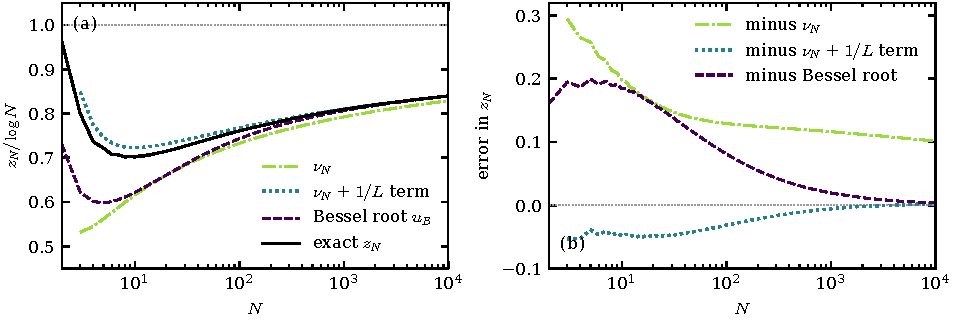
\includegraphics{figures/crossing}
\caption{(a) The scaled crossing $z_N/\log N$ (solid) and the same quantity from the Bessel root
$u_B$ of Theorem~\ref{thm:bessel} (dashed), from $\nu_N$ of \eqref{eq:secondorder} (through the
constant) and from $\nu_N+(\frac14\log L-\frac12c_0+\frac18)/L$ of \eqref{eq:thirdorder} (with the
$1/L$ term). The ratio
tends to $1$ very slowly. (b) The exact $z_N$ minus each approximation.}
\label{fig:crossing}
\end{figure}

\section{The crossing of every bin}\label{sec:allbin}

The same question makes sense for each bin: at which $p$ is bin $k$ exactly
as likely as an endpoint? Figure~\ref{fig:allbin} shows the answer for 3
values of $N$. The crossing $1-p_{a,N-a}$ decreases as the bin moves in from
the edge, from order $N^{-1/2}$ next to the edge to order $(\log N)/N$ in the
middle. This section proves this picture.

\subsection{Ordering the crossings}\label{sec:allbin-order}

Let $a,b\ge1$ be integers, $N=a+b$ and $p>0$, and recall that
$S_{a,b}(u)=P_N(a)/P_N(0)$ with $u=(1-p)/p$. Theorem~\ref{thm:pmf} and
$\binom{m-1}{r+1}=\frac{m-1-r}{r+1}\binom{m-1}{r}$ for $m=a,b$ give
\begin{equation}\label{eq:allbin-polynomial}
 S_{a,b}(u)=\sum_{r\ge0}\binom{a-1}{r}\binom{b-1}{r}
 \Bigl(2u^{2r+1}+\frac{N-2-2r}{r+1}u^{2r+2}\Bigr).
\end{equation}
Its coefficients are nonnegative, as $N-2-2r\ge|b-a|$ for $r<\min(a,b)$, and
the linear one is $2$. So there is a unique $u_{a,b}>0$ with
$S_{a,b}(u_{a,b})=1$, and $p_{a,b}=1/(1+u_{a,b})$. As $S_{a,b}(u)\ge2u$, we
have $u_{a,b}\le\frac12$ and $p_{a,b}\in[\frac23,1)$, with $p_{a,b}=\frac23$
only for $a=b=1$.

\begin{proposition}[ordering the crossings]\label{prop:allbin-order}
If $a<b-1$, then
\[
 u_{a+1,b-1}<u_{a,b},\qquad p_{a+1,b-1}>p_{a,b}.
\]
Also $p_{a,b+1}>p_{a,b}$ for all positive $a,b$. In fact the corresponding
inequalities between the polynomials $S_{a+1,b-1}$ and $S_{a,b}$, or
$S_{a,b+1}$ and $S_{a,b}$, hold coefficientwise, with at least one strict
coefficient.
\end{proposition}

In words: a bin closer to the middle, or in a longer row, needs a larger $p$
to fall to the endpoint height.

\begin{proof}
For fixed $N$ and $r\le a-1$,
$\binom{a-1}{r}\binom{b-1}{r}=(r!)^{-2}\prod_{j=0}^{r-1}(a-1-j)(b-1-j)$, a
product of positive factors. Each factor grows when $(a,b)$ becomes
$(a+1,b-1)$, by $(a-j)(b-2-j)-(a-1-j)(b-1-j)=b-a-1>0$. The even multiplier
$(N-2-2r)/(r+1)$ is unchanged, and it is nonnegative where either product is
nonzero, since then $r\le a$ and $N-2-2r\ge b-a-2\ge0$. New summands are
nonnegative, and the cubic coefficient grows strictly, from $2(a-1)(b-1)$ to
$2a(b-2)$. Increasing $b$ with $a$ fixed increases the binomial coefficients
of Theorem~\ref{thm:pmf}, and the quadratic coefficient $N-2$ strictly. A
polynomial with nonnegative coefficients that dominates another
coefficientwise, strictly somewhere, is strictly larger at every $u>0$, so its
root is smaller.
\end{proof}

The ordering of the bin heights below also follows from the interior
log-concavity of Dekking and Kong~\cite[Proposition~4.3]{dekkingkong2011}. We
use the coefficients because they also give the strict gap in the next
proposition.

\begin{proposition}[adjacent bins and global extrema]\label{prop:adjacent}
For $N\ge2$ and $0<p<1$, an adjacent bin has the same probability as an
endpoint precisely at
\[
p_N^{\mathrm{adj}}=\frac{1+\sqrt{N-1}}{2+\sqrt{N-1}}.
\]
For $0<p<1$, the endpoints are the least likely bins if
$p<p_N^{\mathrm{adj}}$, bins $1$ and $N-1$ are if $p>p_N^{\mathrm{adj}}$, and
they tie at equality. For $N\ge4$, the central crossing satisfies
$p_N>p_N^{\mathrm{adj}}$. At $p=p_N$, the middle and endpoints attain the
global maximum and bins $1,N-1$ attain the global minimum. For $N=2,3$,
$p_N=p_N^{\mathrm{adj}}$ and every bin ties at the crossing.
\end{proposition}

So at the central crossing the row has the shape of a W: high at the 2 ends
and in the middle, and lowest next to the ends.

\begin{proof}
By \eqref{eq:allbin-polynomial}, $S_{1,N-1}(u)=2u+(N-2)u^2$, with positive
root $u^{\mathrm{adj}}=1/(1+\sqrt{N-1})$. This gives $p_N^{\mathrm{adj}}$ and
the sign change. For $0<p<1$ we have $P_N(k)=P_N(0)S_{k,N-k}(u)$ with
$P_N(0)>0$, so if $1\le k<N-k-1$ Proposition~\ref{prop:allbin-order} gives
$P_N(k)<P_N(k+1)$. By symmetry the middle is the largest interior bin and bins
$1,N-1$ are the smallest, which gives the claims about the least likely bins.
For $N\ge4$ the cubic coefficient $2(\lfloor N/2\rfloor-1)(\lceil N/2\rceil-1)$
of $S_N$ is positive, so $2u_N+(N-2)u_N^2<S_N(u_N)=1$, hence
$u_N<u^{\mathrm{adj}}$ and $p_N>p_N^{\mathrm{adj}}$. At $p_N$ the middle ties
with the endpoints, which gives the global maximum, and bins $1,N-1$ are below
the endpoints, which gives the global minimum. For $N=2,3$ we have
$S_N=S_{1,N-1}$, and symmetry gives the ties.
\end{proof}

So $1-p_N^{\mathrm{adj}}\sim N^{-1/2}$, much larger than
$1-p_N\sim(\log N)/N$. The reason is simple. Away from the ends the single
$\sR$ of bin $1$ needs 2 switches, so $S_{1,N-1}\approx Nu^2$ reaches $1$ only
at $u\approx N^{-1/2}$. (At $p=0$ and $p=1$ there are also ties between bins of
probability $0$.)

\subsection{A Bessel estimate uniform in the bin}\label{sec:allbin-bessel}

Bin $a$ has about $(a^r/r!)(b^r/r!)$ words with $r$ runs of each letter, each
of weight about $u^{2r}$. The sum depends only on $abu^2$, so a bin near the
edge acts like the middle of a shorter row with $\sqrt{ab}$ in place of $N/2$.
Put
\[
 s=\sqrt{ab},\quad A=\frac{ab}{a+b},\quad
 c=\frac{a+b}{2\sqrt{ab}},\quad
 \eta=\frac1c,\quad x=su,\quad J_c(x)=I_0(2x)+cI_1(2x),
\]
and $\widehat S_{a,b}(u)=2uJ_c(su)$. Here $c\ge1$ and $0<\eta\le1$, with
$\eta=1$ exactly when $a=b$.

\begin{theorem}[uniform estimate for every bin]\label{thm:allbin-bessel}
For all positive integers $a,b$ and all $u>0$,
\begin{equation}\label{eq:allbin-bessel}
 0\le 1-\frac{S_{a,b}(u)}{\widehat S_{a,b}(u)}
 \le \frac{(a+b)u^2}{2}+u
 =\frac{x^2}{2A}+\frac xs.
\end{equation}
In particular, for fixed $N$ and $u$ the bound does not depend on the bin.
The inequality still holds when the right side exceeds 1, but then it gives no
lower bound on $S_{a,b}$.
\end{theorem}

In words, every bin is a Bessel function of $\sqrt{ab}\,u$ up to a relative
error of at most $Nu^2/2+u$, which is $O(L^2/N)$ for every bin at once when
$u$ is about $L/N$. The proof is that of Theorem~\ref{thm:bessel}(i), with the
2 letters weighted by $a$ and $b$.

\begin{proof}
Let $U_r=U_r(a)$ and $V_r=U_r(b)$ as in Lemma~\ref{lem:clipped}(b), and
$H=1/a+1/b=1/A$. Lemma~\ref{lem:clipped}(a), applied to the $2r$ clipped
factors of $U_rV_r$, gives
\begin{equation}\label{eq:allbin-odd-deficit}
 0\le1-U_rV_r\le\frac H2r(r+1).
\end{equation}
The same argument for the weighted average
$E_r=(aU_{r+1}V_r+bU_rV_{r+1})/(a+b)$ gives
\begin{align}
 0\le1-E_r
 &\le\frac{(r+1)(r+2)}{a+b}
 +\frac{r(r+1)}{2(a+b)}\Bigl(\frac ab+\frac ba\Bigr)\notag\\
 &=\frac H2r(r+1)+\frac{2(r+1)}{a+b}.\label{eq:allbin-even-deficit}
\end{align}
Since $\binom{a-1}r=a^rU_r/r!$, \eqref{eq:allbin-polynomial} becomes
\begin{equation}\label{eq:allbin-normalized-series}
 S_{a,b}(u)=2u\Bigl[
 \sum_{r\ge0}\frac{x^{2r}}{(r!)^2}U_rV_r
 +c\sum_{r\ge0}\frac{x^{2r+1}}{r!(r+1)!}E_r\Bigr],
\end{equation}
and dropping $U_rV_r$ and $E_r$ gives $\widehat S_{a,b}(u)$. So by
Lemma~\ref{lem:clipped}(c), with $I_j=I_j(2x)$,
$(\widehat S_{a,b}-S_{a,b})/(2u)$ lies between $0$ and
\[
 \frac H2(x^2I_0+xI_1+cx^2I_1)+\frac{2c\,xI_0}{a+b}
 =\Bigl(\frac{x^2}{2A}+\frac xs\Bigr)J_c(x),
\]
since $H/2=c/s=1/(2A)$ and $2c/(a+b)=1/s$. Divide by $\widehat S_{a,b}/(2u)=J_c(x)$.
\end{proof}

To turn this into a bound on the crossing, let $x_{a,b}=su_{a,b}$ and let
$x_B$ be the positive root of
\begin{equation}\label{eq:allbin-bessel-root}
 G_\eta(x_B)=A,\qquad
 G_\eta(x)=x\{I_1(2x)+\eta I_0(2x)\}.
\end{equation}
Differentiating term by term gives
\begin{equation}\label{eq:allbin-logderivative}
 G_\eta'(x)-2G_\eta(x)
 =2x(1-\eta)\{I_0(2x)-I_1(2x)\}+\eta I_0(2x)\ge0,
\end{equation}
since $I_0(2x)-I_1(2x)=\frac1\pi\int_0^\pi e^{2x\cos\theta}(1-\cos\theta)\,d\theta>0$
by \cite[Eq.~10.32.3]{dlmf}. So $(\log G_\eta)'\ge2$ for $x>0$ and
$0\le\eta\le1$, and $x_B$ is unique.

\begin{corollary}[quantitative crossing bound]\label{cor:allbin-root-bound}
We have $x_{a,b}\ge x_B$. If
\[
 \delta_{a,b}=\frac{x_{a,b}^2}{2A}+\frac{x_{a,b}}s<1,
\]
then
\begin{equation}\label{eq:allbin-root-bound}
 0\le x_{a,b}-x_B\le-\tfrac12\log(1-\delta_{a,b}).
\end{equation}
\end{corollary}

\begin{proof}
Since $c\eta=1$ and $2c/s=1/A$, we have $\widehat S_{a,b}(u)=G_\eta(su)/A$. At
the crossing $S_{a,b}=1$, so Theorem~\ref{thm:allbin-bessel} gives
$A\le G_\eta(x_{a,b})\le A/(1-\delta_{a,b})$. As $G_\eta(x_B)=A$, this gives
$x_{a,b}\ge x_B$, and integrating $(\log G_\eta)'\ge2$ from $x_B$ to
$x_{a,b}$ gives \eqref{eq:allbin-root-bound}. This is the argument of
Theorem~\ref{thm:bessel}(ii). For even $N$ and $a=b$ the 2 statements
coincide, since then $\eta=1$, $s=h$ and $2G_1=F$.
\end{proof}

\begin{remark}[Jacobi polynomials]\label{rem:jacobi}
The Bessel forms in this paper are classical in another guise: they come from
the confluence of Jacobi, Laguerre and Bessel functions near the point $1$.
For $a\le b$ and $0\le t<1$,
\[
 \sum_{r\ge0}\binom{a-1}{r}\binom{b-1}{r}t^r
 ={}_2F_1(1-a,1-b;1;t)
 =(1-t)^{a-1}P_{a-1}^{(0,\,b-a)}\Bigl(\frac{1+t}{1-t}\Bigr),
\]
and for $b>a$ and $0\le u<1$,
\[
 \sum_{r\ge0}\binom{a-1}{r}\binom{b-1}{r+1}u^{2r+2}
 =\frac{(b-1)u^2}{a}(1-u^2)^{a-1}P_{a-1}^{(1,\,b-a-1)}\Bigl(\frac{1+u^2}{1-u^2}\Bigr).
\]
Near $1$, Jacobi polynomials of large degree behave like Bessel functions (the
Mehler--Heine formula \cite[Eq.~18.11.5]{dlmf}), and
Elliott~\cite{elliott1971} gives expansions in modified Bessel functions
uniform near $1$. For fixed $a$ and $y=bu^2$, as $b\to\infty$,
\cite[Eq.~18.7.21]{dlmf} turns the last sum into
$(y/a)L_{a-1}^{(1)}(-y)=H_a(y)$ of \eqref{eq:edge-polynomial}, and the other
terms tend to $0$. Temme~\cite{temme1990} gives asymptotic estimates of
Gegenbauer, Laguerre and Jacobi polynomials. But Elliott's expansions have
fixed parameters and no error bounds, while here $b-a$ can be as large as
$N-2$, and Theorem~\ref{thm:allbin-bessel} gives an explicit relative error at
every $N$.
\end{remark}

\subsection{Every growing distance from an edge}\label{sec:allbin-growing}

The Bessel root satisfies an equation of the form
$z+\frac12\log z=\ell+C+B/z+\dots$. The next lemma inverts such equations.

\begin{lemma}[inverting $z+\frac12\log z$]\label{lem:inversion}
Fix $K>0$. There is a constant $C_K$ with the following property. Let $z\ge1$
and $\ell\ge2$, and suppose that $z+\tfrac12\log z=\ell+C+B/z+\omega$ with
$|C|,|B|\le K$ and $|\omega|\le1$. Then
\[
\Bigl|z-\ell+\tfrac12\log\ell-C-\frac{\frac14\log\ell-\frac12C+B}{\ell}\Bigr|
\le C_K\Bigl(\frac{(\log\ell)^2}{\ell^2}+|\omega|\Bigr).
\]
\end{lemma}

\begin{proof}
Put $w=z-\ell$. As $z\ge1$, $\log z\ge0$ and $|B/z|\le K$, so $z\le\ell+2K+1$
and $|w|\le2K+1+\frac12\log(\ell+2K+1)=O_K(\log\ell)$. This proves the claim
for $\ell$ bounded in terms of $K$, since then both sides are $O_K(1)$ and
$(\log\ell)^2/\ell^2$ is bounded below. For larger $\ell$ we have
$|w|\le\ell/2$, so $\log z=\log\ell+w/\ell+O((w/\ell)^2)$ and
$B/z=B/\ell+O_K(|w|/\ell^2)$, and
$w=C-\frac12\log\ell-w/(2\ell)+B/\ell+\omega+O_K((\log\ell)^2/\ell^2)$. This
gives first $w=d+O_K(\log\ell/\ell+|\omega|)$ with $d=C-\frac12\log\ell$, and
then, putting this back into the term $w/(2\ell)$,
$w=d+(B-d/2)/\ell+O_K((\log\ell)^2/\ell^2+|\omega|)$.
\end{proof}

\begin{theorem}[uniform crossing expansion]\label{thm:allbin-expansion}
Let $1\le a\le b$, and put
\[
 \ell=\log A,\qquad
 C(\eta)=\tfrac12\log(8\pi)-\log(1+\eta),\qquad
 B(\eta)=\frac{3-\eta}{8(1+\eta)}.
\]
As $a\to\infty$, uniformly over $b\ge a$,
\begin{align}
 2\sqrt{ab}\,u_{a,b}
 ={}&\ell-\tfrac12\log\ell+C(\eta)\notag\\
 &+\frac{\tfrac14\log\ell-\tfrac12C(\eta)+B(\eta)}{\ell}
 +O\left(\frac{(\log\ell)^2}{\ell^2}+\frac{(\log a)^2}{a}\right).
 \label{eq:allbin-expansion}
\end{align}
That is, there are $a_0$ and $C$ such that the error term is at most $C$
times the bracket for all $a\ge a_0$ and all $b\ge a$. The same holds with
$1-p_{a,b}$ in place of $u_{a,b}$.
\end{theorem}

In words: a bin far from both edges crosses where $2\sqrt{ab}\,u$ is about
$\log A$, with $A=ab/(a+b)$ half the harmonic mean of $a$ and $b$. There is no
condition on how $a$ compares with $N$, so this covers a bin at distance
$\sqrt N$ from the edge as well as the middle. The idea of the proof:
Corollary~\ref{cor:allbin-root-bound} moves the problem to the Bessel root
$x_B$, and the large-argument form of $I_0$ and $I_1$ turns
\eqref{eq:allbin-bessel-root} into an equation that Lemma~\ref{lem:inversion}
solves.

\begin{proof}
Here $a/2\le A\le a$, $s\ge a$ and $0<\eta\le1$.

\emph{Step 1: the crossing is at $x_{a,b}\le\log a$.} At $x=\log a$ the bound
of Theorem~\ref{thm:allbin-bessel} is at most $2(\log a)^2/a$, while
$G_\eta(x)/A\ge xI_1(2x)/a\to\infty$, both uniformly in $b$. So $S_{a,b}>1$
there, and $x_{a,b}\le\log a$ for all $a\ge a_0$ and all $b\ge a$. Then
$\delta_{a,b}\le2(\log a)^2/a$, and Corollary~\ref{cor:allbin-root-bound}
gives
\begin{equation}\label{eq:allbin-root-error}
 x_{a,b}-x_B=O((\log a)^2/a).
\end{equation}

\emph{Step 2: the Bessel root.} Write $z=2x_B$, so $z\to\infty$ as
$A\to\infty$, uniformly in $\eta$. By the large-argument form of $I_0$ and
$I_1$ \cite[Eq.~10.40.1]{dlmf},
$I_1(z)+\eta I_0(z)=(1+\eta)e^z(2\pi z)^{-1/2}(1-B(\eta)/z+O(z^{-2}))$
uniformly in $0\le\eta\le1$. Taking logarithms in
\eqref{eq:allbin-bessel-root} gives
$z+\frac12\log z=\ell+C(\eta)+B(\eta)/z+O(z^{-2})$. As $|C(\eta)|\le2$ and
$0<B(\eta)\le\frac38$, Lemma~\ref{lem:inversion} with $K=2$ expands $z$.

\emph{Step 3: back to the crossing.} By \eqref{eq:allbin-root-error} the
expansion moves to $2x_{a,b}=2\sqrt{ab}\,u_{a,b}$. Finally
$2s(u-u/(1+u))\le2x^2/s=O((\log a)^2/a)$ at $u=u_{a,b}$, which gives the same
expansion for $1-p_{a,b}=u_{a,b}/(1+u_{a,b})$.
\end{proof}

Hence, uniformly in $b$,
\begin{equation}\label{eq:allbin-leading}
 1-p_{a,b}\sim\frac{\log a}{2\sqrt{ab}}
 \qquad(a\to\infty,\ b\ge a).
\end{equation}
If $a=o(b)$, then $\eta\to0$ and
$\log A=\log a+o(1)$, so
\begin{equation}\label{eq:allbin-growing-edge}
 2\sqrt{ab}(1-p_{a,b})
 =\log a-\tfrac12\log\log a+\tfrac12\log(8\pi)+o(1).
\end{equation}
If $a/N\to\alpha\in(0,\frac12]$ at any rate, then
\[
 2\sqrt{a(N-a)}(1-p_{a,N-a})
 =\log N-\tfrac12\log\log N+\log\{\alpha(1-\alpha)\}+C(2\sqrt{\alpha(1-\alpha)})+o(1).
\]
At the center, $a=b=N/2$ gives $A=N/4$ and $\eta=1$, and changing from
$\log A$ to $\log N$ recovers \eqref{eq:thirdorder}.

\begin{figure}[t]
\centering
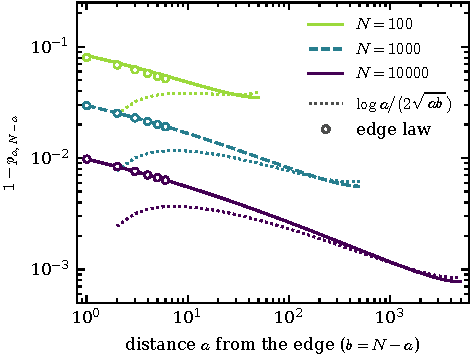
\includegraphics{figures/allbin}
\caption{The crossing $1-p_{a,N-a}$ of each bin against its distance $a$
from the nearer edge, for $N=100$, $1000$ and $10^4$. The dotted lines are the
leading law \eqref{eq:allbin-leading}, and the circles are the edge law
\eqref{eq:edge-q-expansion} for $a\le6$. The right end of each line is the
central crossing $1-p_N$.}
\label{fig:allbin}
\end{figure}

\subsection{Fixed bins and the Laguerre edge law}\label{sec:allbin-edge}

Now let $a$ be fixed and $b\to\infty$. A run of $\sR$'s away from the ends
needs 2 switches, which gives a factor $u^2$, and it can go in about $b$
places. So the right variable is $y=bu^2$. Define
\begin{equation}\label{eq:edge-polynomial}
 H_a(y)=\sum_{r=0}^{a-1}\binom{a-1}{r}\frac{y^{r+1}}{(r+1)!}
 =\frac ya L_{a-1}^{(1)}(-y),
\end{equation}
with the standard Laguerre polynomial $L_{a-1}^{(1)}$. Let $y_a$ be the
positive root of $H_a(y_a)=1$ and $c_a=\sqrt{y_a}$. Then $y_1=1$,
$y_2=\sqrt3-1$, and $y_a$ decreases strictly in $a$, by coefficient
comparison.

\begin{theorem}[fixed-edge expansion]\label{thm:edge-laguerre}
For each fixed positive integer $a$, as $b\to\infty$,
\begin{equation}\label{eq:edge-crossing-expansion}
 u_{a,b}=\frac{c_a}{\sqrt b}-\frac1b
 +\frac{\gamma_a}{b^{3/2}}+O_a(b^{-2}),
\end{equation}
where
\[
 \gamma_a=
 \frac{1+y_a+(y_a+y_a^2/2)H_a''(y_a)/H_a'(y_a)}{2c_a}.
\]
Thus the second coefficient in the odds expansion is $-1$ for every fixed
bin. For the switching probability,
\begin{equation}\label{eq:edge-q-expansion}
 1-p_{a,b}=\frac{c_a}{\sqrt b}-\frac{1+c_a^2}{b}+O_a(b^{-3/2}).
\end{equation}
\end{theorem}

In words, bin $a$ near the edge crosses at odds about $\sqrt{y_a/b}$, and the
first correction does not depend on $a$. For bin $1$ this gives
$u_{1,b}=b^{-1/2}-b^{-1}+b^{-3/2}+\dots$, the expansion of the exact root
$1/(1+\sqrt b)$ of Proposition~\ref{prop:adjacent}.

\begin{proof}
Put $\epsilon=b^{-1/2}$, $y=bu^2$ and $V_r=U_r(b)$. For $b\ge a$,
\eqref{eq:allbin-polynomial} reads
\begin{align}
 S_{a,b}(u)={}&2\sqrt{y/b}\sum_r\binom{a-1}{r}\frac{y^r}{r!}V_r\notag\\
 &+\frac yb\sum_r\binom{a-1}{r+1}\frac{y^r}{r!}V_r
 +y\sum_r\binom{a-1}{r}\frac{y^r}{(r+1)!}V_{r+1}.
 \label{eq:edge-exact-series}
\end{align}
These sums have at most $a$ terms, and with $V_r=1$ they are $H_a'(y)$,
$H_a''(y)$ and $H_a(y)$. Expanding $V_r=1-r(r+1)/(2b)+O_a(b^{-2})$ and using
$\sum_r(r+1)(r+2)\binom{a-1}{r}\frac{y^{r+1}}{(r+1)!}=y^2H_a''(y)+2yH_a'(y)$
gives, uniformly near $y=y_a$,
\begin{align}
 S_{a,b}(u)={}&H_a(y)+2\sqrt y\,H_a'(y)\epsilon\notag\\
 &+\{(y-y^2/2)H_a''(y)-yH_a'(y)\}\epsilon^2+O_a(\epsilon^3).
 \label{eq:edge-implicit-expansion}
\end{align}
With $b=\epsilon^{-2}$ the right side of \eqref{eq:edge-exact-series} is
analytic in $(\epsilon,y)$ near $(0,y_a)$, and $H_a'(y_a)>0$. So the
implicit-function theorem gives an analytic solution
$y(\epsilon)=y_a+d_1\epsilon+d_2\epsilon^2+O_a(\epsilon^3)$ of $S_{a,b}=1$,
and by the uniqueness of the crossing it is the value of $y$ at $u=u_{a,b}$.
Matching coefficients in \eqref{eq:edge-implicit-expansion} gives $d_1=-2c_a$
and $d_2=2+y_a+(y_a+y_a^2/2)H_a''(y_a)/H_a'(y_a)$. Expanding $u=\epsilon\sqrt y$
and then $u/(1+u)$ proves both expansions.
\end{proof}

For large $a$ the Laguerre root $y_a$ should obey the growing-distance law
\eqref{eq:allbin-growing-edge}. The next theorem shows this.

\begin{theorem}[matching the edge and Bessel regimes]\label{thm:edge-matching}
For every positive integer $a$ and every $x>0$,
\begin{equation}\label{eq:laguerre-bessel-bound}
 0\le1-\frac{aH_a(x^2/a)}{xI_1(2x)}\le\frac{x^2}{2a}.
\end{equation}
Consequently, with $\ell=\log a$ and $C_0=\tfrac12\log(8\pi)$, as $a\to\infty$,
\begin{align}
 2\sqrt{a y_a}
 ={}&\ell-\tfrac12\log\ell+C_0\notag\\
 &+\frac{\tfrac14\log\ell-\tfrac12C_0+3/8}{\ell}
 +O\left(\frac{(\log\ell)^2}{\ell^2}+\frac{(\log a)^2}{a}\right).
 \label{eq:edge-matching-expansion}
\end{align}
\end{theorem}

\begin{proof}
With $U_r=U_r(a)$, $aH_a(x^2/a)=x\sum_{r\ge0}U_rx^{2r+1}/(r!(r+1)!)$, so
Lemma~\ref{lem:clipped}(b) and the second identity of
Lemma~\ref{lem:clipped}(c) give \eqref{eq:laguerre-bessel-bound}. Put
$x_a=\sqrt{ay_a}$, so $aH_a(x_a^2/a)=a$, and $x_a<\log a$ for large $a$ by
\eqref{eq:laguerre-bessel-bound}. So $a\le G_0(x_a)\le a/(1-x_a^2/(2a))$, and
as in Corollary~\ref{cor:allbin-root-bound}, $x_a-x_0=O((\log a)^2/a)$, where
$G_0(x_0)=a$. So $z=2x_0$ satisfies
$z+\frac12\log z=\ell+C_0+3/(8z)+O(z^{-2})$ by \cite[Eq.~10.40.1]{dlmf}, as in
the proof of Theorem~\ref{thm:allbin-expansion} with $\eta=0$ and $A=a$, and
Lemma~\ref{lem:inversion} gives the expansion.
\end{proof}

Figure~\ref{fig:allbin} compares these laws with the exact crossings.

\subsection{The moving boundary layer}\label{sec:allbin-layer}

The crossings also give the shape of a whole row at odds $u=v_N>0$. Between
the central crossing ($v_N$ about $(\log N)/N$) and the adjacent one ($v_N$
about $N^{-1/2}$), the middle is above the endpoints and a layer of bins next
to each edge is below them. How thick is this layer? Let
\[
 \mathcal L_N=\#\{1\le k\le\lfloor N/2\rfloor:P_N(k)<P_N(0)\}.
\]

\begin{corollary}[boundary-layer width]\label{cor:boundary-layer}
Suppose that, as $N\to\infty$,
\[
 \Omega_N=\frac1{\sqrt N\,v_N}\longrightarrow\infty,
 \qquad \frac{\log\Omega_N}{Nv_N}\longrightarrow0.
\]
Then
\begin{equation}\label{eq:boundary-layer-width}
 \mathcal L_N\sim\Omega_N^2\log^2\Omega_N
 =\frac{\log^2(1/(\sqrt N\,v_N))}{Nv_N^2}.
\end{equation}
In particular, if $v_N=N^{-\gamma}$ with $1/2<\gamma<1$, then
\[
 \mathcal L_N\sim(\gamma-\tfrac12)^2N^{2\gamma-1}\log^2N.
\]
By symmetry, the total number of interior bins below the endpoint height
is $2\mathcal L_N$ for all sufficiently large $N$.
\end{corollary}

\begin{proof}
Set $d_N=\Omega_N^2\log^2\Omega_N$. Then $d_N\to\infty$ and
$d_N/N=(\log\Omega_N/(Nv_N))^2\to0$. Fix $\varepsilon\in(0,1)$ and integers
$a_\pm=(1\pm\varepsilon)d_N+O(1)$. Then $\log a_\pm\sim2\log\Omega_N$ and
$\sqrt{a_\pm(N-a_\pm)}\,v_N\sim\sqrt{1\pm\varepsilon}\,\log\Omega_N$, so
\eqref{eq:allbin-leading} gives
$u_{a_\pm,N-a_\pm}/v_N\to1/\sqrt{1\pm\varepsilon}$. Bin $k$ is below the
endpoint exactly when $v_N<u_{k,N-k}$, and $u_{k,N-k}$ decreases strictly for
$k\le N/2$ by Proposition~\ref{prop:allbin-order}. So
$a_-\le\mathcal L_N<a_+$ for large $N$, and we let $\varepsilon\downarrow0$.
Finally $\mathcal L_N=o(N)$, so the reflected intervals are disjoint.
\end{proof}

\section{Periodic boundaries and the crossing window}\label{sec:periodicwindow}

There are 2 ways to make Kagey's board periodic, and they are different. On a
cylinder the ball moves around a circle of pegs, and its position becomes
uniform (Remark~\ref{rem:cyl}). Here we keep the line of bins but close the
sequence of steps into a loop, so that the last step also interacts with the
first. This is the periodic Ising chain, with weight proportional to
$\exp(J\sum_{i=1}^N\sigma_i\sigma_{i+1})$, $\sigma_{N+1}=\sigma_1$ and again
$u=e^{-2J}$. Antal, Droz and R\'acz~\cite{antal2004} give its magnetization law
at a fixed scale, and Dantchev and Rudnick~\cite{dantchev2022} give exact
coefficients. We ask how much the closing bond moves the central crossing, and
then look at the row near the crossing under both boundaries.

Write $R^{\mathrm F}_{N,k}=S_{k,N-k}$ and $R^{\mathrm P}_{N,k}$ for the
bin-to-endpoint ratios under free and periodic boundaries. Put $a=k$, $b=N-k$
and $s=\sqrt{ab}$. The classical cyclic count is
\begin{equation}\label{eq:periodicratio}
R^{\mathrm P}_{N,k}(u)=\sum_{r=1}^{\min(a,b)}\frac Nr
 \binom{a-1}{r-1}\binom{b-1}{r-1}u^{2r}.
\end{equation}
To see this, note that a cyclic word with $a$ letters $\sR$ and $b$ letters
$\sL$ switches an even number $2r$ of times and has $r$ runs of each letter.
Choose compositions of $a$ and of $b$ into $r$ positive runs and a position for
the start of a distinguished run of $\sR$'s, and divide by the $r$ choices of
that run. The normalization of the periodic measure cancels in the ratio. In
particular $R^{\mathrm P}_{N,1}=Nu^2$, which gives the adjacent crossing
$J=(\log N)/4$ of Stepanyan et~al.\@~\cite{stepanyan2024}. Every interior
ratio increases strictly from $0$ to $\infty$ in $u>0$, and the ratios
increase strictly toward the middle, apart from the symmetric middle tie, by
the coefficient comparison of Proposition~\ref{prop:allbin-order}.

\begin{theorem}[periodic relative error]\label{thm:periodic-bessel}
For $N\ge2$, $1\le k\le N-1$, and $u>0$, define
\[
\widehat R^{\mathrm P}_{N,k}(u)=\frac{Nu}{\sqrt{k(N-k)}}
 I_1\!\left(2u\sqrt{k(N-k)}\right).
\]
Then
\begin{equation}\label{eq:periodicbound}
0\le1-\frac{R^{\mathrm P}_{N,k}(u)}{\widehat R^{\mathrm P}_{N,k}(u)}
\le\frac{Nu^2}{2}.
\end{equation}
\end{theorem}

In words, under periodic boundaries every bin is a single Bessel function
$I_1$, with the same kind of error as in Theorem~\ref{thm:allbin-bessel}.

\begin{proof}
Put $x=su$, $A=ab/N$, $U_r=U_r(a)$ and $V_r=U_r(b)$. Shifting the index in
\eqref{eq:periodicratio} gives
$R^{\mathrm P}_{N,k}(u)=(Nu/s)\sum_{r\ge0}U_rV_rx^{2r+1}/(r!(r+1)!)$, so the
ratio to $\widehat R^{\mathrm P}_{N,k}$ is an average of the $U_rV_r$ with
weights $x^{2r+1}/(r!(r+1)!)$, whose sum is $I_1(2x)$. By
\eqref{eq:allbin-odd-deficit}, $0\le1-U_rV_r\le r(r+1)/(2A)$, and the second
identity of Lemma~\ref{lem:clipped}(c) bounds the deficit by
$x^2/(2A)=Nu^2/2$.
\end{proof}

We can guess the next theorem. A cyclic word switches an even number of times,
so only $I_1$ appears in the periodic approximation, while the free words that
start and end on different letters give the extra $I_0$ term of the free one.
As $I_0\approx I_1$ for large arguments, the free ratio is about twice the
periodic one near the crossing. Both grow like $e^{Nu}$, so the periodic
crossing needs $Nu$ about $\log2$ larger. The same factor $2$ appears at a
fixed scale $T$ in the endpoint atoms $1/(2\cosh T)$ (periodic) and $e^{-T}/2$
(free) of Antal, Droz and R\'acz~\cite[Eqs.~(37) and~(47)]{antal2004}, while
their densities at zero magnetization agree to leading order.

\begin{theorem}[periodic crossing and boundary shift]\label{thm:periodic-crossing}
Let $u_N^{\mathrm P}$ be the positive root of $R^{\mathrm P}_{N,m_N}(u)=1$,
let $p_N^{\mathrm P}=1/(1+u_N^{\mathrm P})$, and let $u_N^{\mathrm F}=u_N$ be
the free central root. Put $c_{\mathrm P}=\tfrac12\log(\pi/2)$. As
$N\to\infty$,
\begin{align}
Nu_N^{\mathrm P}
 &=L-\tfrac12\log L+c_{\mathrm P}
 +\frac{\tfrac14\log L-\tfrac12c_{\mathrm P}+\tfrac38}{L}
 +O\!\left(\frac{(\log L)^2}{L^2}\right),\label{eq:periodicasym}\\
N(u_N^{\mathrm P}-u_N^{\mathrm F})
 &=\log2+\frac{\tfrac14-\tfrac12\log2}{\log N}
 +o(1/\log N).\label{eq:boundaryshift}
\end{align}
Replacing $Nu_N^{\mathrm P}$ by $N(1-p_N^{\mathrm P})$ preserves
\eqref{eq:periodicasym}. At the periodic crossing the coupling
$J_N^{\mathrm P}=-\frac12\log u_N^{\mathrm P}$ satisfies
\begin{equation}\label{eq:isingtemperature}
J_N^{\mathrm P}
=\tfrac12(\log N-\log\log N)
+\frac{\tfrac14\log\log N-\tfrac12c_{\mathrm P}}{\log N}
+O\!\left(\frac{(\log\log N)^2}{(\log N)^2}\right).
\end{equation}
\end{theorem}

In words, closing the loop makes every nonconstant word switch an even number
of times, so the endpoints become relatively more likely, and the periodic
chain needs about $\log2$ more expected switches before the middle catches up
with them. Since $c_{\mathrm P}=c_0+\log2$, the periodic
expansion is the free one shifted by $\log2$, with $\frac38$ in place of
$\frac18$ in the $1/L$ term.

\begin{proof}
\emph{Step 1: the first order.} At the middle $2s=N+O(1/N)$. At
$u=(1\pm\epsilon)L/N$ with fixed $\epsilon\in(0,1)$ the bound of
Theorem~\ref{thm:periodic-bessel} tends to $0$, and the large-argument form of
$I_1$ makes $\widehat R^{\mathrm P}$ tend to $\infty$ with the plus sign and
to $0$ with the minus sign. Since $R^{\mathrm P}_{N,m_N}$ increases in $u$, we
get $Nu_N^{\mathrm P}\sim L$.

\emph{Step 2: the crossing equation.} Write $z=Nu_N^{\mathrm P}$. At the root
$\log\widehat R^{\mathrm P}=O(L^2/N)$ by \eqref{eq:periodicbound}. Replacing
the argument $2su$ by $z$ changes it by $O(L/N^2)$, and
$I_1(z)=e^z(2\pi z)^{-1/2}(1-3/(8z)+O(z^{-2}))$~\cite[Eq.~10.40.1]{dlmf}. So
\[
z+\tfrac12\log z=L+c_{\mathrm P}+\frac3{8z}+O(z^{-2}+L^2/N),
\]
and Lemma~\ref{lem:inversion} with $\ell=L$, $C=c_{\mathrm P}$ and
$B=\frac38$ gives \eqref{eq:periodicasym}. As $N(u-u/(1+u))=O(L^2/N)$ for
$Nu=O(L)$, it also holds for $N(1-p_N^{\mathrm P})$.

\emph{Step 3: the shift and the coupling.} By \eqref{eq:zN},
$Nu_N=z_N+O(L^2/N)$. Subtracting \eqref{eq:thirdorder}, where
$c_0=c_{\mathrm P}-\log2$ and the correction is $\frac18$, gives
\eqref{eq:boundaryshift}, even with error $O((\log L)^2/L^2)$. Finally
$J=-\frac12\log u=\frac12(L-\log z)$, and
$\log z=\log L-(\frac12\log L-c_{\mathrm P})/L+O((\log L)^2/L^2)$ gives
\eqref{eq:isingtemperature}.
\end{proof}

Stepanyan et~al.\@~\cite[Eq.~(16)]{stepanyan2024} approximate the periodic
crossing by $\beta J\approx(2\log N-1)/5$, and their Fig.~1(b) fits the line
$\beta J\approx0.3864\log N-0.21055$. At $N=10^5$ the exact periodic crossing
is $J=4.576$ (their $\beta J$). Their Eq.~(16) gives $4.405$, their line gives
$4.238$, and \eqref{eq:isingtemperature} without its error term gives $4.578$.
The line is accurate for $10\le N\le100$ (at $N=100$ it gives $1.569$ and the
exact value is $1.574$), but it has no $\log\log N$ term.

Now we look at the whole row near the crossing. How many bins are above the
endpoints just past the crossing, and how does their height fall off away from
the middle? The factor $e^{-2y^2}$ in the next theorem is easy to guess.
Moving $yN/\sqrt{\log N}$ away from the middle multiplies the Bessel argument
by $2\sqrt{k(N-k)}/N\approx1-2y^2/\log N$. The argument is about $\log N$, so
it drops by about $2y^2$, and the ratio, which grows like $e$ to the argument,
drops by about the factor $e^{-2y^2}$.

\begin{theorem}[spatial crossing window]\label{thm:critical-window}
Let $X\in\{\mathrm F,\mathrm P\}$ and let $u_N^X$ be its exact central
crossing. For fixed real $t,y$ set
\[
u=u_N^X+\frac tN,\qquad
k_N(y)=\operatorname{nint}\!\left(\frac N2+\frac{yN}{\sqrt{\log N}}\right),
\]
where either nearest-integer convention may be used. Then, as $N\to\infty$,
uniformly on compact sets of $(t,y)$,
\begin{equation}\label{eq:criticalprofile}
R^X_{N,k_N(y)}(u_N^X+t/N)\longrightarrow e^{t-2y^2}.
\end{equation}
If $M_N^X(t)$ is the number of interior bins with probability strictly above
the endpoint probability at that parameter, then
\begin{equation}\label{eq:criticalcount}
\frac{\sqrt{\log N}}N M_N^X(t)\longrightarrow\sqrt{2\max(t,0)}.
\end{equation}
\end{theorem}

In words, the crossing window has width about $1/N$ in $u$ and about
$N/\sqrt{\log N}$ in space, and inside it the row is a Gaussian bump times
$e^t$. A weak limit theorem cannot give this, since it says nothing about a
single bin such as the endpoint.

\begin{proof}
\emph{Step 1: the profile.} Put $\delta=k/N-\frac12$ and
$\eta=2\sqrt{k(N-k)}/N=\sqrt{1-4\delta^2}$. For the stated rounding and
bounded $y$,
\[
\eta=1-\frac{2y^2}{L}+O\Bigl(L^{-2}+\frac1{N\sqrt L}\Bigr),
\qquad Nu_N^X=L+O(\log L).
\]
So the Bessel argument $Nu\eta$ at $(u,k)$ is $Nu_N^X+t-2y^2+o(1)$, uniformly
on the compact set. By Theorems~\ref{thm:allbin-bessel}
and~\ref{thm:periodic-bessel} both ratios are within relative error
$O(L^2/N)$ of their Bessel forms, and $I_0(z)$ and $I_1(z)$ equal
$e^z(2\pi z)^{-1/2}(1+O(1/z))$~\cite[Eq.~10.40.1]{dlmf}, so the prefactors
relative to their central values tend to $1$ uniformly. The change of argument
gives $e^{t-2y^2}$, and the exact central ratio is $1$, which proves
\eqref{eq:criticalprofile}.

\emph{Step 2: the count.} The interior ratios increase toward the middle. If
$t\le0$, the central ratio is at most $1$, so no interior bin is above the
endpoint. Let $t>0$ and $0<\epsilon<\sqrt{t/2}$. By Step~1, for large $N$ the
bins at scaled distance less than $\sqrt{t/2}-\epsilon$ are above the endpoint
and those at distance $\sqrt{t/2}+\epsilon$ are below, and by monotonicity so
are all farther bins. Count the bins in between, divide by $N/\sqrt L$ and let
$\epsilon\downarrow0$. Rounding changes the count by $O(1)$.
\end{proof}

Figure~\ref{fig:window} shows the exact ratios at $N=10^6$.

\begin{figure}[t]
\centering
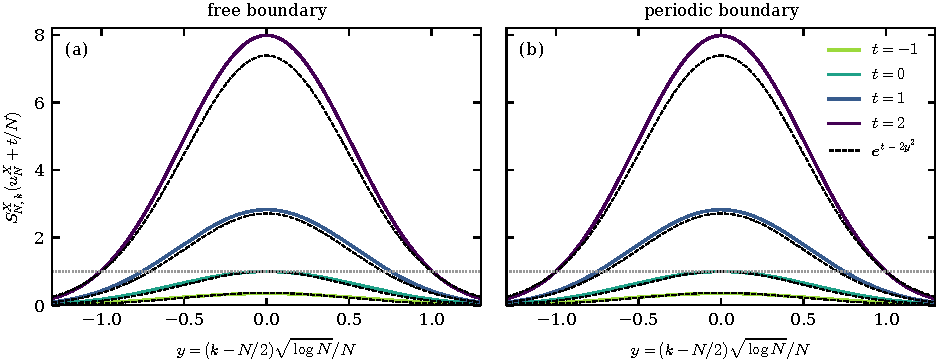
\includegraphics{figures/window}
\caption{The exact ratios $R^X_{N,k}(u_N^X+t/N)$ at $N=10^6$ for free (a) and
periodic (b) boundaries, with the limit $e^{t-2y^2}$ of
Theorem~\ref{thm:critical-window} (dashed). Here $y=(k-N/2)\sqrt{\log N}/N$,
and the bins above the dotted line are above the endpoint height. The
convergence is slow, and at $t=2$ and $y=0$ the relative error is still $0.08$.}
\label{fig:window}
\end{figure}

\section{A uniform local law}\label{sec:llt}

So far we compared each bin with an endpoint. Now we approximate $P_N(k)$ itself by a single
formula, uniformly in $q\le\frac12$, from the diffusive regime ($q$ fixed) to the ballistic
regime ($T=Nq$ bounded). Throughout, $n_1=k-1$, $n_2=N-k-1$ and $n_{\min}=\min(n_1,n_2)$.

\begin{theorem}[a difference of 2 binomials]\label{thm:llt-identity}
Let $N\ge2$, $1\le k\le N-1$ and $0<q<1$. Let $Y_1\sim\mathrm{Bin}(n_1,q)$ and
$Y_2\sim\mathrm{Bin}(n_2,q)$ be independent, and put $D=Y_1-Y_2$. Then
\begin{equation}\label{eq:llt-identity}
P_N(k)=\frac q2\bigl[2\Prob(D=0)+\Prob(D=1)+\Prob(D=-1)\bigr].
\end{equation}
\end{theorem}

\begin{proof}
We rewrite Theorem~\ref{thm:pmf}, where $a-1=n_1$ and $b-1=n_2$. Note that
$\Prob(Y_1=r)\Prob(Y_2=r')=\binom{n_1}r\binom{n_2}{r'}q^{r+r'}p^{N-2-r-r'}$. The term $j=2r+1$ of
Theorem~\ref{thm:pmf} is $\binom{n_1}r\binom{n_2}rp^{N-2-2r}q^{2r+1}=q\Prob(Y_1=r)\Prob(Y_2=r)$,
and summing over $r$ gives $q\Prob(D=0)$. The term $j=2r+2$ is
\[
\tfrac12\Bigl[\tbinom{n_1}{r+1}\tbinom{n_2}r+\tbinom{n_1}r\tbinom{n_2}{r+1}\Bigr]p^{N-3-2r}q^{2r+2}
=\tfrac q2\bigl[\Prob(Y_1=r+1)\Prob(Y_2=r)+\Prob(Y_1=r)\Prob(Y_2=r+1)\bigr],
\]
and summing over $r$ gives $\frac q2[\Prob(D=1)+\Prob(D=-1)]$.
\end{proof}

For $k=1$ we have $n_1=0$ and $D=-Y_2$, so $\Prob(D=0)=p^{N-2}$, $\Prob(D=-1)=(N-2)qp^{N-3}$ and
$\Prob(D=1)=0$. By \eqref{eq:llt-identity} and symmetry,
\begin{equation}\label{eq:llt-edge}
P_N(1)=P_N(N-1)=qp^{N-2}+\tfrac12(N-2)q^2p^{N-3}.
\end{equation}
With $P_N(0)=P_N(N)=\frac12p^{N-1}$, the 4 bins $0,1,N-1,N$ are exact, and from now on $N\ge4$
and $2\le k\le N-2$.

Next we tilt $D$ to mean $0$. For $s>0$ put
\[
r_1=\frac{qs}{p+qs},\qquad r_2=\frac q{ps+q},\qquad v_i=r_i(1-r_i),\qquad
\Lambda(s)=(p+qs)^{n_1}(p+q/s)^{n_2}.
\]
Under the tilted law $\Prob_s$, $Y_1\sim\mathrm{Bin}(n_1,r_1)$ and
$Y_2\sim\mathrm{Bin}(n_2,r_2)$ are independent, and $\Prob(D=j)=\Lambda(s)s^{-j}\Prob_s(D=j)$
(Lemma~\ref{lem:llt-tilt}). Since $n_1,n_2\ge1$, there is a unique $s>0$ with $n_1r_1=n_2r_2=:m$,
so that $\E_sD=0$ (Lemma~\ref{lem:llt-saddle}). We fix this $s$, let $x=n_1v_1+n_2v_2$ be the
variance of $D$ under $\Prob_s$, and define
\begin{equation}\label{eq:llt-U}
U_N(k)=\frac q2\Lambda(s)e^{-x}\bigl[2I_0(x)+(s+s^{-1})I_1(x)\bigr].
\end{equation}
At the center of an even row, $n_1=n_2$ gives $s=1$, $r_1=r_2=q$ and $\Lambda=1$, so
\begin{equation}\label{eq:llt-center}
U_N(N/2)=q\,e^{-x}\bigl(I_0(x)+I_1(x)\bigr),\qquad x=(N-2)pq.
\end{equation}

Note that by \eqref{eq:llt-identity} and the tilt,
$P_N(k)=\frac q2\Lambda(s)\bigl[2\Prob_s(D=0)+s^{-1}\Prob_s(D=1)+s\Prob_s(D=-1)\bigr]$. The law
$e^{-x}I_{|j|}(x)$ on $\Z$ is the symmetric Skellam law, the law of a difference of 2 independent
Poisson variables with mean $x/2$, and it has mean $0$ and variance $x$. So $U_N(k)$ replaces the
tilted $D$ by the Skellam law with the same mean and variance. This law is exact for a Poisson
difference, which $D$ resembles when $q$ is small, and close to Gaussian when $x$ is large. At the
center $D$ is a sum of $N/2-1$ independent variables with $\Prob(\pm1)=pq$, and replacing it by
this Skellam law is the approximation that \v{C}ekanavi\v{c}ius and
Liaudanskait\.{e}~\cite[Eq.~(3)]{cekanavicius2024} attribute to Presman. The tilt extends it off
the center.

Let $\kappa=1-\cos t$ and write $\langle h\rangle$ for the average of $h(t)$ against the density
proportional to $e^{x\cos t}$ on $[-\pi,\pi]$. With $\mathcal R=\mathcal R(x)=I_1(x)/I_0(x)$,
Lemma~\ref{lem:llt-moments} gives
\[
\langle\kappa^2\rangle=2-2\mathcal R-\frac{\mathcal R}x,\qquad
\langle\kappa^3\rangle=4-4\mathcal R-\frac{3\mathcal R}x-\frac{2\mathcal R}{x^2}+\frac1x.
\]
Put $V=n_1v_1^2+n_2v_2^2$ and $M=m\max(r_1,r_2)$.

\begin{theorem}[uniform local law]\label{thm:llt}
Let $N\ge4$, $2\le k\le N-2$ and $0<q<1$. Then $P_N(k)=U_N(k)(1+\theta)$ with
\[
|\theta|\le\mathcal E:=\frac1{\mathcal R(x)}\Bigl[\Bigl(4V+\frac{64}3M\Bigr)\langle\kappa^2\rangle
+\frac{1024}9M^2\langle\kappa^3\rangle\Bigr].
\]
\end{theorem}

We sketch the proof. By Fourier inversion, $P_N(k)$ and $U_N(k)$ are
$\frac q2\Lambda(s)\frac1{2\pi}\int_{-\pi}^{\pi}f\omega\,dt$ with
$\omega(t)=2+se^{it}+s^{-1}e^{-it}$, where $f$ is $\chi(t)=\E_se^{itD}$ for $P_N(k)$ and the
Skellam characteristic function $g(t)=e^{x(\cos t-1)}$ for $U_N(k)$. Since
$|1-r+re^{it}|^2=1-2v\kappa=e^{-2v\kappa}(1+O(v^2\kappa^2))$ with $v=r(1-r)$, $|\chi|\le g$
and $g-|\chi|=O(V\kappa^2)\,g$. The phase of $\chi$ has no linear term since $\E_sD=0$, so it is
$O(M|t|^3)$. Hence $|\theta|$ is at most a constant times
$\bigl((V+M)\langle\kappa^2\rangle+M^2\langle\kappa^3\rangle\bigr)/\mathcal R(x)$, where
$\langle\kappa^j\rangle=O(\min(1,x^{-j}))$ and $1/\mathcal R(x)\le1+2/x$. The proof with explicit
constants is in Appendix~\ref{app:llt}.

\begin{corollary}\label{cor:llt}
Let $N\ge4$, $2\le k\le N-2$ and $0<q\le\frac12$, and put $r_{\max}=\max(r_1,r_2)$. Then
\[
|\theta|\le\min\Bigl\{\frac{22334}{n_{\min}},\ 221\,r_{\max}+5825\,r_{\max}^2\Bigr\}.
\]
Also $r_{\max}\le\delta_T:=2T/\sqrt N+4T^2/N$, so $|\theta|\le221\,\delta_T+5825\,\delta_T^2$ for
every bin $2\le k\le N-2$. At the center of an even row, $r_{\max}=q$ and $n_{\min}=N/2-1$.
\end{corollary}

So the relative error tends to $0$ uniformly in $0<q\le\frac12$ as $n_{\min}\to\infty$, and
uniformly over $2\le k\le N-2$ as $T/\sqrt N\to0$, which covers the ballistic regime $T=O(1)$ up
to the edges. The constants are crude. The largest $n_{\min}|\theta|$ we observed is $0.686$, at
$N=10^4$ and $q=\frac12$. It is the largest over $2\le k\le400$ at $N=10^4$ with $q=\frac12$ or
$0.3$, and over every bin of our grid with $N\le1000$ and $10^{-5}\le q\le\frac12$. The first
bound has the constant $22334$ instead, so it exceeds $1$ unless $n_{\min}>22334$. Near an edge the largest error we
observed is $|\theta|=0.1617$ ($k=3$, $N=10^4$, $q=\frac12$), an observation and not a bound. For
$q>\frac12$ Theorem~\ref{thm:llt} still holds, but $\mathcal E$ need not be small, and a uniform
form is open. Near $q=1$ the symmetric kernel fails once $n_1\ne n_2$. We found $\theta=0.578$ at
the middle bin $k=50$ of the odd row $N=101$ with $q=0.999$, while $\theta\approx0$ at $N=100$,
$k=50$.

Replacing $e^{-x}I_j(x)$ in \eqref{eq:llt-U} by $(2\pi x)^{-1/2}$ gives the Gaussian saddle point
$G_N(k)=\frac q2\Lambda(s)(2+s+s^{-1})(2\pi x)^{-1/2}$. We also define the transfer-matrix
form $\mathrm{TM}_N=2(2\pi(N-1)p/q)^{-1/2}$, the Gaussian local form for $\Prob(X_N=0)$ with the
variance $(N-1)p/q$ that $\lambda_+^{N-1}$ gives in the proof of Theorem~\ref{thm:clt}. The
factor $2$ is the span of the lattice of $X_N=2k-N$.

\begin{proposition}[Gaussian saddle points]\label{prop:llt-gauss}
Fix an even $N\ge4$. As $q\to0$,
\[
\frac{P_N(N/2)}q\to1,\qquad
\frac{G_N(N/2)}{P_N(N/2)}\sim\frac2{\sqrt{2\pi(N-2)q}}\to\infty,\qquad
\frac{\mathrm{TM}_N}{P_N(N/2)}\sim\frac2{\sqrt{2\pi(N-1)q}}\to\infty.
\]
\end{proposition}

\begin{proof}
The term $j=1$ of Theorem~\ref{thm:pmf} is $qp^{N-2}$ and the other terms are $O(q^2)$, so
$P_N(N/2)=q+O(q^2)$. At the center $s=1$, $\Lambda=1$ and $x=(N-2)pq$, so
$G_N(N/2)=2q/\sqrt{2\pi(N-2)pq}$. Also $\mathrm{TM}_N=2q/\sqrt{2\pi(N-1)pq}$. Let $q\to0$.
\end{proof}

More generally, since $P_N(N/2)/q\to1$, any approximation $A_N(q)$ of the center with
$A_N(q)/q\to\infty$ has relative error $P_N(N/2)/A_N(q)-1\to-1$. Both saddle points are of this
kind. We make no claim about other Gaussian forms. The Bessel form avoids this because
$e^{-x}I_j(x)$ is exact for the Poisson difference that $D$ approaches in the ballistic regime.

\begin{remark}[the center crossing]\label{rem:llt-center}
For even $N\ge4$ let $\mathcal G(q)$ be the logarithm of the ratio of $U_N(N/2)$ to
$P_N(0)=\frac12p^{N-1}$. By $I_0'=I_1$, $I_1'=I_0-I_1/x$ \cite[Eqs.~10.29.2, 10.29.3]{dlmf} and
$I_1\le I_0$, we get $\mathcal G'(q)\ge\frac1{2pq}+\frac{N-1}p>N-1$ on $(0,\frac12]$. Also $\mathcal G\to-\infty$ as
$q\to0$ and $\mathcal G(\frac12)\ge(N-1)\log2-\frac{N-2}4>0$, so $\mathcal G$ has a unique root $q_U$ there, an
approximate crossing. In Table~\ref{tab:llt-center}, which is purely numerical, the relative error
of $q_U$ is 16 to 36 times smaller than that of the Bessel root $u_B$ of Theorem~\ref{thm:bessel}.
Put $\vartheta_N=221q_N+5825q_N^2$. If $\vartheta_N<1$, Corollary~\ref{cor:llt} gives
$|\mathcal G(q_N)|\le\vartheta_N/(1-\vartheta_N)$, and the mean value theorem gives
$|q_U-q_N|\le\vartheta_N/((1-\vartheta_N)(N-1))$. By our computation $\vartheta_N\ge1$ for every
even $N<1454$, and beyond it this bound is weaker than Theorem~\ref{thm:bessel}(ii) at every $N$
we computed.
\end{remark}

\begin{table}[ht]
\centering\small
\begin{tabular}{@{}rcccc@{}}
\toprule
$N$ & $p_N$ & $q_U/q_N-1$ & $u_B/u_N-1$ & ratio\\
\midrule
100 & 0.9649663263 & $-1.477\times10^{-3}$ & $-2.39\times10^{-2}$ & 0.062\\
400 & 0.9881246429 & $-3.083\times10^{-4}$ & $-7.61\times10^{-3}$ & 0.041\\
1600 & 0.9962346137 & $-6.469\times10^{-5}$ & $-2.31\times10^{-3}$ & 0.028\\
\bottomrule
\end{tabular}
\caption{The root $q_U$ of $U_N(N/2)=P_N(0)$ against the Bessel root $u_B$ of
Theorem~\ref{thm:bessel}. The ratio is $(q_U/q_N-1)/(u_B/u_N-1)$. Numerical values, not bounds.}
\label{tab:llt-center}
\end{table}

At the center our kernel is the Skellam law of \cite[Eq.~(3)]{cekanavicius2024}, as noted above.
\v{C}ekanavi\v{c}ius and
Liaudanskait\.{e}~\cite{cekanavicius2024} and \v{C}ekanavi\v{c}ius and
Vellaisamy~\cite{cekanavicius2010} give total-variation, local and Wasserstein bounds with
unspecified absolute constants for chains outside our regime. One is a symmetric 3-state chain
whose step is $0$ with probability at least $\frac{14}{15}$. The other is a 2-state chain with
$\Prob(1\mid1)\le\frac12$, and some of its bounds also need $\Prob(1\mid0)\le\frac1{30}$. Neither
allows both states to persist, as our $p\to1$ does. Jensen~\cite{jensen2013}
conditions the count $S_n$ on $0<S_n<n$ and patches small tilted variances, and his relative
error stays bounded (about $0.18$, found partly by numerics) but does not tend to $0$. In the
literature we searched we did not find a tilted Skellam kernel off the center with a relative
local error, explicit constants and uniformity in $q\le\frac12$.


\section{Verification}\label{sec:verify}

The checks for all 4 papers are described in \texttt{SUPPLEMENT.md}, in the
Problem 131 folder of \url{https://github.com/apemm/Kagey-Problems}, together
with the manuscript source and the recorded results. The scripts are
standard-library Python, and \texttt{python -B verify\_all.py --paper a} runs
the ones for this paper (\texttt{--full} adds 2 long runs of about 21
minutes). They check the exact law, the lattice-path counts, the orderings,
the Bessel bounds and the asymptotic formulas, and where possible each
reported number is computed in 2 independent ways. Apart from
Remark~\ref{rem:sign}, which is computer-assisted throughout, a proof rests on
only 2 computations. These are the integer certificates for $N\le174$ in
Theorem~\ref{thm:every-n} and Proposition~\ref{prop:crossing-eq}, made and
rechecked by \texttt{verify\_every\_n.py} and
\texttt{verify\_every\_n\_guards.py}, and the evaluation at $N=2774$ in
Corollary~\ref{cor:every-n}(d). Before the main computations (the
monotonicity and Bessel-ratio checks, the every-$N$ certificates and the local
law) we wrote
predictions and conditions that would refute them in \texttt{ledger.md},
\texttt{paperA/data/ledger\_every\_n.md} and \texttt{paperA/data/ledger\_llt.md}, and we
recorded the outcomes there. Some small-$N$ predictions for
Theorem~\ref{thm:every-n} were not blind, as the ledger says. The Lean~4
proofs are in \texttt{lean/PaperA}, and \texttt{lean/README.md} lists them.
They include the exact law, the numerator tables, the variance and the normal
limit, the orderings of the crossings, the uniform Bessel bounds and root
comparisons, the leading terms $1-p_N\sim(\log N)/N$ and
$2\sqrt{ab}\,u_{a,b}\sim\log a$, the finite parts of the edge and periodic
results, Lemmas~\ref{lem:bracket} and~\ref{lem:bessel-bounds} and
Theorem~\ref{thm:every-n} for every $N\ge2$. The finite parts are the
polynomial $H_a$ and its root $y_a$, the exact series
\eqref{eq:edge-exact-series}, the cyclic count \eqref{eq:periodicratio} and
the adjacent periodic crossing. For Theorem~\ref{thm:edge-laguerre} only the
algebra of the coefficients is in Lean. For $N\le174$ the Lean kernel checks
the same certificates in exact integer arithmetic, with its own rational
bounds on $\zeta_N$, so the whole theorem is proved in Lean.
\texttt{lean/build-log.txt} shows that every theorem uses only the standard
axioms. Remarks~\ref{rem:bernoulli}, \ref{rem:cyl}, \ref{rem:jacobi}
and~\ref{rem:sign}, Corollary~\ref{cor:every-n} beyond part~(a),
Proposition~\ref{prop:crossing-eq}, Lemma~\ref{lem:inversion},
Theorem~\ref{thm:allbin-expansion} beyond its leading term, the expansions
of Theorem~\ref{thm:edge-laguerre}, the expansion
\eqref{eq:edge-matching-expansion} of Theorem~\ref{thm:edge-matching},
Theorem~\ref{thm:periodic-crossing}, even its leading term,
Corollary~\ref{cor:boundary-layer}, Theorem~\ref{thm:critical-window} and
Section~\ref{sec:llt} are not in Lean.

\paragraph{Acknowledgment.}
The Lean code for this paper was generated by AI. AI was also used to revise
some of the writing and to help cross-verify the code.

\appendix
\section{The crossing at every \texorpdfstring{$N$}{N}}\label{app:every-n}

This appendix proves Lemma~\ref{lem:bessel-bounds}, the analytic half of
Theorem~\ref{thm:every-n}, the identity behind the certificates and
Proposition~\ref{prop:crossing-eq}. The letters $U$, $U'$, $W$, $W'$, $r$,
$r'$, $t$, $t'$, $\tau$, $\kappa$, $m$, $B$, $D$, $\beta$, $\Delta$ and
$\delta$ are local to this appendix (each is defined where it first shows up).
We round every decimal constant in the safe direction, namely so that the
inequality it enters stays true.

\subsection{Proof of Lemma~\ref{lem:bessel-bounds}}

For integer $n$, $I_n(z)=\frac1\pi\int_0^\pi e^{z\cos t}\cos(nt)\,dt$
\cite[Eq.~10.32.3]{dlmf}, so
$I_0(z)+I_1(z)=\frac1\pi\int_0^\pi e^{z\cos t}(1+\cos t)\,dt$. Substitute
$s=1-\cos t$, so that $\sin t=\sqrt{s(2-s)}$ and $1+\cos t=2-s$, and then
$s=v/z$. This gives
\begin{equation}\label{eq:E-integral}
\cE(z)=\frac1{\sqrt\pi}\int_0^{2z}e^{-v}v^{-1/2}\sqrt{1-\frac v{2z}}\,dv .
\end{equation}
On $[0,1]$ we have $\sqrt{1-y}=1-\sum_{k\ge1}c_ky^k$ with every $c_k>0$,
$c_1=\frac12$ and $c_2=\frac18$, and $\sum_kc_k=1$ by monotone convergence as
$y\uparrow1$. So $\sum_{k\ge3}c_k=\frac38$, and $y^k\le y^3$ gives
$\sum_{k\ge3}c_ky^k\le\frac38y^3$. Hence, for $0\le y\le1$,
\[
g_-(y):=1-\frac y2-\frac{y^2}8-\frac{3y^3}8\le\sqrt{1-y}\le1-\frac y2-\frac{y^2}8
\le g_+(y):=1-\frac y2-\frac{y^2}8+\frac{y^3}8 .
\]
The cubic $g_-$ decreases and $g_-(1)=0$, so $g_-\le0$ on $[1,\infty)$. Also
$8g_+(y)=(y-2)^2(y+1)+2(y-1)^2+2>0$ for $y\ge-1$. Put $y=v/(2z)$ in
\eqref{eq:E-integral}, replace $\sqrt{1-y}$ by $g_\pm$ and extend the integral
to $\infty$. The added piece is at most $0$ with $g_-$ and at least $0$ with
$g_+$, so the lower bound survives with $g_-$ and the upper with $g_+$. Since
$\frac1{\sqrt\pi}\int_0^\infty e^{-v}v^{k-1/2}\,dv=\Gamma(k+\frac12)/\Gamma(\frac12)$
equals $1,\frac12,\frac34,\frac{15}8$ for $k=0,1,2,3$, the two bounds integrate
to the two sides of the lemma. The bound $\cE\le1$ follows in the same way from
$\sqrt{1-y}\le1$. Finally $-\frac3{128z^2}+\frac{15}{512z^3}\le0$ exactly when
$z\ge\frac54$.

\subsection{Proof of Theorem~\ref{thm:every-n} for \texorpdfstring{$N\ge175$}{N >= 175}}

\emph{Step 1. Bounds that hold for every $\zeta\ge4$.} Fix $N\ge175$ and write
$\zeta=\zeta_N$, $U=\zeta+\frac1{8\zeta}$, $r=U/N$ and
$n(\zeta)=\sqrt{8\zeta/\pi}\,e^\zeta$. Then $n(\zeta_N)=N$ by
\eqref{eq:zetaN}, and $\zeta\ge4$ since $n(4)<175$. For $k=1,2,3$ the function
$U^k/n(\zeta)$ decreases on $[4,\infty)$, because its logarithmic derivative is
$k(1-\frac1{8\zeta^2})/U-1-\frac1{2\zeta}<\frac kU-1<0$. The same holds for
$U^4/n$, since $U>4$, and for $\zeta/n$ and $\zeta^2/n$. The values at
$\zeta=4$ give, for every $\zeta\ge4$,
\[
r\le0.023135,\quad\frac{U^2}N\le0.093262,\quad\frac{U^3}N\le0.375960,\quad
\frac{U^4}N\le1.51559,\quad\frac{\zeta(\zeta+1)}N\le0.114776 .
\]

\emph{Step 2. The upper bound.} Let $W=U/(1-r)$, so that $NW/(N+W)=U$, and let
$\delta=W(W+2)/(2N)$. By Lemma~\ref{lem:bracket}(b) and \eqref{eq:bracket-log}
it suffices to show that $G_U:=\psi(W)-\psi(\zeta)+\log \cE(W)+\log(1-\delta)>0$.
We bound the three parts from below. First,
$\psi(W)-\psi(\zeta)=(W-U)+(U-\zeta)+\frac12\log\frac U\zeta+\frac12\log\frac WU$,
where $W-U=\frac{Ur}{1-r}$, $U-\zeta=\frac1{8\zeta}$,
$\log\frac U\zeta=\log(1+\frac1{8\zeta^2})\ge\frac1{8\zeta^2}-\frac1{128\zeta^4}$
and $\log\frac WU=-\log(1-r)\ge r$. Second, Lemma~\ref{lem:bessel-bounds} gives
$\cE(W)\ge1-t$ with $t=\frac1{8W}+\frac3{128W^2}+\frac{45}{512W^3}$. Since
$W\ge U\ge\zeta$ and
$\frac1{8U}=\frac1{8\zeta}-\frac1{8\zeta(8\zeta^2+1)}\le\frac1{8\zeta}-\frac1{64\zeta^3}+\frac1{512\zeta^5}$,
we get
$t\le\tau:=\frac1{8\zeta}+\frac3{128\zeta^2}+\frac{37}{512\zeta^3}+\frac1{512\zeta^5}$
and $\log \cE(W)\ge\log(1-\tau)\ge-\tau-\frac{\tau^2}{2(1-\tau)}$. Third,
$\delta=\frac{Ur}{2(1-r)^2}+\frac r{1-r}$ and
$\log(1-\delta)\ge-\delta-\frac{\delta^2}{2(1-\delta)}$. Adding the three parts
gives $G_U\ge B+D$, where $B$ collects the terms in $\zeta$ alone and $D$ the
terms with a factor $r$,
\[
B=\frac5{128\zeta^2}-\frac{37}{512\zeta^3}-\frac1{256\zeta^4}-\frac1{512\zeta^5}-\frac{\tau^2}{2(1-\tau)},\qquad
D=\frac r{2(1-r)}\Bigl(\frac{U(1-2r)}{1-r}-1-r\Bigr)-\frac{\delta^2}{2(1-\delta)} .
\]
Both $\zeta\tau$ and $\tau$ decrease in $\zeta$, so $\zeta^2B$ increases. At
$\zeta=4$ we have $\zeta\tau=0.135384$, $\tau=0.033846$ and
$\zeta^2B=0.011236$. Hence $B>0$. In $D$ the bracket is at least
$4.03125(1-0.023683)-1.023135>2.912$, so the first term of $D$ is at least
$1.456\,r$. Write $\delta=rm$ with $m=\frac U{2(1-r)^2}+\frac1{1-r}$. Then
$\delta\le0.07255$ and
$rm^2=\frac{U^3}{4N(1-r)^4}+\frac{U^2}{N(1-r)^3}+\frac r{(1-r)^2}\le0.2276$, so
$\frac{\delta^2}{2(1-\delta)}=r\cdot\frac{rm^2}{2(1-\delta)}\le0.1228\,r$.
Hence $D\ge1.33\,r>0$. So $G_U>0$ and $z_N<U$.

\emph{Step 3. The lower bound.} Let $\varepsilon=\varepsilon_N$,
$U'=U-\varepsilon$, $r'=U'/N$ and $W'=U'/(1-r')$, so that
$NW'/(N+W')=U'$. By Step~1, $\varepsilon\le0.114776+\frac1{256}<0.1187$, so
$U'\ge\zeta-0.1187\ge3.88$ and $W'\ge U'$. By Lemma~\ref{lem:bracket}(a)
and \eqref{eq:bracket-log} it suffices to show that
$G_{U'}:=\psi(W')-\psi(\zeta)+\log \cE(W')<0$. We bound the two parts from above.
First,
$\psi(W')-\psi(\zeta)=(U'-\zeta)+\frac{U' r'}{1-r'}+\frac12\log\frac{U'}\zeta-\frac12\log(1-r')$,
where $U'-\zeta=\frac1{8\zeta}-\varepsilon$,
$\frac12\log\frac{U'}\zeta\le\frac12(\frac{U'}\zeta-1)=\frac1{16\zeta^2}-\frac\varepsilon{2\zeta}$
and $-\frac12\log(1-r')\le\frac{r'}{2(1-r')}$. The two terms in $r'$ add up to
$\frac{U'^2+U'/2}{N(1-r')}$. Second, Lemma~\ref{lem:bessel-bounds} gives
$\cE(W')\le1-t'$ with
$t'=\frac1{8W'}+\frac3{128W'^2}-\frac{15}{512W'^3}\in(0,1)$, so
$\log \cE(W')\le-t'$. Here $\frac1{8W'}=\frac1{8U'}-\frac1{8N}$. Write
$U'=\zeta(1+\kappa)$ with $\kappa=\frac1{8\zeta^2}-\frac\varepsilon\zeta$.
Then $\frac1{U'}\ge\frac{1-\kappa}\zeta$, so
$-\frac1{8W'}\le-\frac1{8\zeta}+\frac1{64\zeta^3}-\frac\varepsilon{8\zeta^2}+\frac1{8N}$.
Next, $x\mapsto x/(1-x/N)$ increases and $U'\le U$, so $W'\le U/(1-r)$ and
$\frac1{W'^2}\ge\frac{(1-r)^2}{\zeta^2(1+\frac1{8\zeta^2})^2}\ge\frac{(1-2r)(1-\frac1{4\zeta^2})}{\zeta^2}$.
Finally $\frac{15}{512W'^3}\le\frac{15}{512U'^3}$. Adding, and using
$\varepsilon(1+\frac1{2\zeta})=\frac{\zeta^2+\frac32\zeta+\frac12}N+\frac1{16\zeta^2}+\frac1{32\zeta^3}$,
we get $G_{U'}\le\beta+\Delta-\frac\varepsilon{8\zeta^2}$ with
\[
\beta=-\frac3{128\zeta^2}(1-2r)\Bigl(1-\frac1{4\zeta^2}\Bigr)+\frac{15}{512U'^3}-\frac1{64\zeta^3},\qquad
\Delta=\frac1N\Bigl(\frac{U'^2+U'/2}{1-r'}+\frac18-\zeta^2-\frac32\zeta-\frac12\Bigr).
\]
For $\beta<0$ it suffices that
$\zeta^2/U'^3\le\frac45(1-2r)(1-\frac1{4\zeta^2})$. The left side is at most
$\zeta^2/(\zeta-0.12)^3\le16/3.88^3<0.274$, since this function decreases for
$\zeta>0.12$ (its logarithmic derivative is $\frac2\zeta-\frac3{\zeta-0.12}<0$
there). The right side is at least $0.8\cdot0.9537\cdot0.9843>0.75$. For
$\Delta<0$, note that $U'\le U$ and $r'\le r$, so
\[
\frac{U'^2+U'/2}{1-r'}\le U^2+\frac U2+\frac{U^3/N+U^2/(2N)}{1-r}
\le\zeta^2+\frac\zeta2+0.2667+0.4326,
\]
using $U^2+\frac U2=\zeta^2+\frac\zeta2+\frac14+\frac1{16\zeta}+\frac1{64\zeta^2}$.
This is less than $\zeta^2+\frac32\zeta+\frac38$ because $\zeta\ge4$. Hence
$G_{U'}<0$ and $z_N>U'$.

The constants were recomputed in 40-digit arithmetic, and as a check outside
the proof we evaluated $\zeta^2B$, $D$, $\beta$ and $\Delta$ on
$\zeta\in[4,60]$ with step $0.001$.

\subsection{The certificates}\label{app:certificates}

Let $c,d>0$ be integers. Multiplying \eqref{eq:SN} by $d^{N-1}$ gives
\[
d^{N-1}S_N(c/d)=\sum_jW(N,m_N,j)\,c^jd^{N-1-j},
\]
an integer. By Theorem~\ref{thm:pmf} it is the sum of
$d^{\rep(w)}c^{\chg(w)}$ over the words $w$ in bin $m_N$, that is, the
numerator $n_N(m_N)$ of Remark~\ref{rem:tables} with $(\alpha,\beta)=(d,c)$.
The recursion \eqref{eq:dp} with the weights $d,c$ in place of $p,q$ and
initial values $1$ computes the same sums. So $S_N(c/d)<1$ exactly when this
integer is less than $d^{N-1}$. This is the identity used in Step~4 of the
proof of Theorem~\ref{thm:every-n}.

\subsection{Proof of Proposition~\ref{prop:crossing-eq}}

\emph{Step 1. An exact formula for $R_N$.} Write $w=w_N$, $z=z_N$,
$\Lambda_N=2\Phi(w)/N$ and $\delta=w(w+2)/(2N)$. At $w=w_N$ the display in the
proof of Lemma~\ref{lem:bracket} gives $1\le\Lambda_N\le1/(1-\delta)$ when
$\delta<1$, and \eqref{eq:bracket-log} gives
$\psi(w)+\log \cE(w)=L+c_0+\log\Lambda_N$. Since $w-z=wz/N$, $w/z=1+w/N$ and
$\frac1{8z}=\frac1{8w}+\frac1{8N}$, the remainder
$R_N=\psi(z)-L-c_0-\frac1{8z}$ is
\begin{equation}\label{eq:RN-formula}
R_N=\log\Lambda_N-\Bigl(\log \cE(w)+\frac1{8w}\Bigr)-\frac1{8N}-\frac{wz}N-\frac12\log\Bigl(1+\frac wN\Bigr).
\end{equation}

\emph{Step 2. The lower bound for $N\ge175$.} By the proof of
Theorem~\ref{thm:every-n}, $3.88\le z\le w\le U/(1-r)$. Note that
$\log\Lambda_N\ge0$ and $-\log \cE(w)\ge-\log(1-\frac1{8w})\ge\frac1{8w}$ by
Lemma~\ref{lem:bessel-bounds}, since $w\ge\frac54$. So
$R_N\ge-\frac{wz+w/2+1/8}N=-\frac{z^2+z/2}{N-z}-\frac1{8N}$. This is at least
$-\frac{z^2+z}N$ as soon as $N\ge\frac{2z^2(z+1)}{z-1/4}$. The right side
increases in $z$ and $z\le U$, so it suffices that
$U^2/N\le\frac{U-1/4}{2(U+1)}$. The left side is at most $0.0933$ and the
right side at least $0.3757$.

\emph{Step 3. The upper bound for $N\ge175$.} Let
$t=\frac1{8w}+\frac3{128w^2}+\frac{45}{512w^3}\le\frac{1.09504}{8w}$, which
holds as $w\ge3.88$. Lemma~\ref{lem:bessel-bounds} and
$-\log(1-t)\le t+\frac{t^2}{2(1-t)}$ give
\[
-\log \cE(w)-\frac1{8w}\le\frac3{128w^2}+\frac{45}{512w^3}+\frac{t^2}{2(1-t)}\le\frac{0.0559}{w^2}
\le\frac{0.0559}{z^2}.
\]
Using $\log\Lambda_N\le\delta+\frac{\delta^2}{2(1-\delta)}$,
$\log(1+x)\ge x-\frac{x^2}2$ and $wz\ge w^2-w^3/N$, the rest of
\eqref{eq:RN-formula} is at most
$-\frac{(w-1/2)^2}{2N}+\frac{w^3+w^2/4}{N^2}+\frac{\delta^2}{2(1-\delta)}$. By
the bounds on $r$ and $U^k/N$ in Step~1 of the previous proof, with
$w\le U/(1-r)$, we have $\frac{w^3+w^2/4}N\le0.4278$ and
$N\frac{\delta^2}{2(1-\delta)}=\frac{(w^4+4w^3+4w^2)/(4N)}{2(1-\delta)}\le0.4945$,
while $\frac{(w-1/2)^2}2\ge5.71$. So the rest is negative and
$R_N\le0.0559/z^2<\frac1{16z^2}$.

\emph{Step 4. The form in $L$ for $N\ge175$.} We have
$z<U=L+c_0-\frac12\log\zeta+\frac1{8\zeta}<L$. Also
$z>\zeta-0.1187\ge\nu_N-0.1187\ge L/2$, because $L-\log L\ge1.18$ for
$L\ge\log175$. Then $\frac1{16z^2}\le\frac1{4L^2}$ and
$\frac{z^2+z}N\le\frac{L^2+L}N$.

\emph{Step 5. $N\le174$.} The function $\phi(z)=\psi(z)-L-c_0-\frac1{8z}$
increases in $z$, and $R_N=\phi(z_N)$, while $\frac1{16z^2}$ and
$-\frac{z^2+z}N$ decrease. So it suffices to check
$\phi(z(c'/d))\le\frac1{16z(c'/d)^2}$ and
$\phi(z(c/d))\ge-\frac{z(c/d)^2+z(c/d)}N$ with the certificates, together with
$z(c/d)\ge L/2$ and, for $N\ge3$, $z(c'/d)\le L$. All hold, and the smallest
gaps are $0.0373$ (upper) and $0.0813$ (lower), both at $N=174$. For $N=2$ we
have $S_2(u)=2u$, so $u_2=\frac12$ and $z_2=\frac23$, and $\frac23<\log2$ is
equivalent to $e^2<8$, which holds since $e^2<2.72^2=7.3984$.

\section{The uniform local law}\label{app:llt}

We keep the notation of Section~\ref{sec:llt}, with $\tilde I_j(x)=e^{-x}I_j(x)$.
The first 2 lemmas set up the tilt, the third writes both $P_N(k)$ and $U_N(k)$
as Fourier integrals, the next 2 compare the modulus and the phase of the 2
integrands, and the last computes the moments of $\kappa$ that appear in the
bound.

\begin{lemma}[tilting]\label{lem:llt-tilt}
For $s>0$ let $Y_1\sim\mathrm{Bin}(n_1,r_1)$ and $Y_2\sim\mathrm{Bin}(n_2,r_2)$ be independent
under $\Prob_s$. Then $\Prob(D=j)=\Lambda(s)s^{-j}\Prob_s(D=j)$ for every $j\in\Z$.
\end{lemma}

\begin{proof}
Note that $\Prob(Y_1=r)s^r=\binom{n_1}r(qs)^rp^{n_1-r}=(p+qs)^{n_1}\Prob_s(Y_1=r)$, and
likewise $\Prob(Y_2=r)s^{-r}=(p+q/s)^{n_2}\Prob_s(Y_2=r)$. Hence
$\Prob(D=j)=s^{-j}\sum_r\Prob(Y_1=r)s^r\,\Prob(Y_2=r-j)s^{j-r}=\Lambda(s)s^{-j}\Prob_s(D=j)$.
\end{proof}

\begin{lemma}[saddle]\label{lem:llt-saddle}
If $n_1,n_2\ge1$, then $\E_sD=n_1r_1-n_2r_2$ increases strictly from $-n_2$ to $n_1$ as $s$ goes
from $0$ to $\infty$. So it vanishes at a unique $s>0$, the positive root of
$n_1ps^2+(n_1-n_2)qs-n_2p=0$, and $s\ge1$ if and only if $n_1\le n_2$.
\end{lemma}

\begin{proof}
Note that $r_1$ increases from $0$ to $1$ and $r_2$ decreases from $1$ to $0$. Clearing
denominators in $n_1qs/(p+qs)=n_2q/(ps+q)$ gives the quadratic, and at $s=1$ the difference is
$(n_1-n_2)q$.
\end{proof}

From now on $2\le k\le N-2$ and $s$ is this root.

\begin{lemma}[Fourier form]\label{lem:llt-fourier}
Let $\chi(t)=\E_se^{itD}=(1-r_1+r_1e^{it})^{n_1}(1-r_2+r_2e^{-it})^{n_2}$,
$g(t)=e^{x(\cos t-1)}$ and $\omega(t)=2+se^{it}+s^{-1}e^{-it}$. Then
\[
P_N(k)=\frac q2\Lambda(s)\frac1{2\pi}\int_{-\pi}^{\pi}\chi\omega\,dt,\qquad
U_N(k)=\frac q2\Lambda(s)\frac1{2\pi}\int_{-\pi}^{\pi}g\omega\,dt.
\]
\end{lemma}

\begin{proof}
By Theorem~\ref{thm:llt-identity} and Lemma~\ref{lem:llt-tilt},
$P_N(k)=\frac q2\Lambda(s)[2\Prob_s(D=0)+s^{-1}\Prob_s(D=1)+s\Prob_s(D=-1)]$, and
$\Prob_s(D=j)=\frac1{2\pi}\int\chi e^{-ijt}dt$. Since $g$ is even and
$I_j(x)=\frac1\pi\int_0^\pi e^{x\cos t}\cos(jt)\,dt$~\cite[Eq.~10.32.3]{dlmf}, we have
$\frac1{2\pi}\int g\,dt=\tilde I_0(x)$ and $\frac1{2\pi}\int ge^{\pm it}dt=\tilde I_1(x)$.
\end{proof}

\begin{lemma}[modulus]\label{lem:llt-modulus}
We have $|\chi|\le g$ and $g-|\chi|\le g\min(1,4\kappa^2V)$.
\end{lemma}

\begin{proof}
Note that $|1-r+re^{\pm it}|^2=1-2r(1-r)\kappa$. Put $f(z)=\sqrt{1-z}\,e^{z/2}$ and
$z_i=2v_i\kappa\in[0,1]$ ($v_i\le\frac14$, $\kappa\le2$). As $x=n_1v_1+n_2v_2$, we get
$|\chi|/g=f(z_1)^{n_1}f(z_2)^{n_2}$. Now $f(0)=1$ and $f'(z)=-\frac z2e^{z/2}(1-z)^{-1/2}\le0$, so
$0\le f\le1$. Also $f(z)\ge1-z^2$, since for $z<1$ this says $e^z\ge(1-z)(1+z)^2=1+z-z^2-z^3$,
which follows from $e^z\ge1+z$. So Lemma~\ref{lem:clipped}(a), with the $n_1+n_2$ numbers
$1-f(z_i)\le z_i^2$, gives $1-|\chi|/g\le n_1z_1^2+n_2z_2^2=4\kappa^2V$.
\end{proof}

\begin{lemma}[phase]\label{lem:llt-phase}
For $|t|<\pi$ write $\chi(t)=|\chi(t)|e^{i\Theta(t)}$ with $\Theta$ continuous and $\Theta(0)=0$.
Then $|\Theta(t)|\le c_\varphi M|t|^3$ with $c_\varphi=128/(3\pi^3)=1.3761\ldots$.
\end{lemma}

\begin{proof}
For $0\le r\le1$ and $|t|<\pi$, $w_r(t)=1-r+re^{it}$ lies on the segment from $1$ to $e^{it}$, so
$w_r\ne0$ and $\arg w_r(t)$ lies between $0$ and $t$. Writing
$w_r(t)=e^{it/2}[\cos\frac t2+i(2r-1)\sin\frac t2]$ gives
$\arg w_r(t)=\frac t2-\arctan\bigl((1-2r)\tan\frac t2\bigr)$. As the factor for $-Y_2$ is
$\overline{w_{r_2}}$, $\Theta=n_1\arg w_{r_1}-n_2\arg w_{r_2}$. Subtracting
$(n_1r_1-n_2r_2)\sin t=0$ gives $\Theta=n_1\varphi(r_1,t)-n_2\varphi(r_2,t)$ with
$\varphi(r,t)=\arg w_r(t)-r\sin t$. Both are odd in $t$, so let $0<t<\pi$. We show that
$0\le\varphi(r,t)\le c_\varphi r^2t^3$.

Put $\tau=\tan\frac t2$, $b_0=1-2r$ and $\gamma(b)=\arctan(b\tau)-b\tau/(1+\tau^2)$. Since
$\frac t2=\arctan\tau$ and $\sin t=2\tau/(1+\tau^2)$, we get $\varphi=\gamma(1)-\gamma(b_0)$. Also
$\gamma$ is odd and $\gamma'(b)=\tau^3(1-b^2)/[(1+\tau^2)(1+b^2\tau^2)]\ge0$ on $[-1,1]$. Hence
\[
\varphi=\frac{\tau^3}{1+\tau^2}\int_{b_0}^1\frac{1-b^2}{1+b^2\tau^2}\,db\ge0,\qquad
\int_{b_0}^1(1-b^2)\,db=4r^2-\tfrac83r^3\le4r^2.
\]
There are 4 cases.
(a) If $t\le\frac\pi2$, then $\tau\le2t/\pi\le1$ by convexity of $\tan$ on $[0,\frac\pi4]$, so
$\varphi\le4r^2\tau^3\le\frac{32}{\pi^3}r^2t^3$.
(b) If $t>\frac\pi2$ and $r\le\frac14$, then $b_0\ge\frac12$, so $1+b^2\tau^2\ge1+\tau^2/4$ and
$\varphi\le16r^2\tau^3/[(1+\tau^2)(4+\tau^2)]$. As $(1+\tau^2)(4+\tau^2)\ge\max(9\tau^2,\tau^4)$,
this is at most $16r^2\min(\tau/9,1/\tau)\le\frac{16}3r^2\le c_\varphi r^2t^3$, as $t^3>\pi^3/8$.
(c) If $t>\frac\pi2$ and $\frac14<r\le\frac12$, then $\gamma(b_0)\ge\gamma(0)=0$, so
$\varphi\le\gamma(1)=\frac12(t-\sin t)\le\frac{t^3}{12}<\frac43r^2t^3$.
(d) If $r>\frac12$, then
$\varphi=\gamma(1)+\gamma(|b_0|)\le2\gamma(1)=t-\sin t\le\frac{t^3}6<\frac23r^2t^3$.
As $\frac{32}{\pi^3},\frac43,\frac23<c_\varphi$, the claim follows. Finally
$\varphi(r_1,t)$ and $\varphi(r_2,t)$ have the same sign, so
$|\Theta|\le\max_in_i\varphi(r_i,t)\le c_\varphi|t|^3\max_in_ir_i^2=c_\varphi M|t|^3$.
\end{proof}

\begin{lemma}[moments]\label{lem:llt-moments}
For every $x>0$, with $\mathcal R=\mathcal R(x)$,
\begin{enumerate}[(i)]
\item $\langle\kappa^2\rangle=2-2\mathcal R-\mathcal R/x$ and
$\langle\kappa^3\rangle=4-4\mathcal R-3\mathcal R/x-2\mathcal R/x^2+1/x$,
\item $1/\mathcal R(x)\le1+2/x$,
\item $\langle\kappa^2\rangle\le\min(\frac32,2/x^2)$ and $\langle\kappa^3\rangle\le\min(\frac52,8/x^3)$.
\end{enumerate}
\end{lemma}

\begin{proof}
(i) Note that $\kappa^2=\frac32-2\cos t+\frac12\cos2t$,
$\kappa^3=\frac52-\frac{15}4\cos t+\frac32\cos2t-\frac14\cos3t$ and
$\langle\cos jt\rangle=I_j(x)/I_0(x)$~\cite[Eq.~10.32.3]{dlmf}. The recurrence
$I_{\nu-1}-I_{\nu+1}=(2\nu/x)I_\nu$~\cite[Eq.~10.29.1]{dlmf} gives $I_2/I_0=1-2\mathcal R/x$ and
$I_3/I_0=\mathcal R-4/x+8\mathcal R/x^2$.

(ii), (iii) By \cite[Eqs.~10.29.2, 10.29.3]{dlmf}, $I_0'=I_1$ and $I_1'=I_0-I_1/x$, so
$\mathcal R'=1-\mathcal R/x-\mathcal R^2$. For a $C^1$ function $h$ put $d_h=1-h/x-h^2-h'$. If
$d_h>0$ on $[x_*,\infty)$ and $\mathcal R(x_*)>h(x_*)$, then $\mathcal R>h$ on $[x_*,\infty)$.
Indeed, at a first $x_1$ with $\mathcal R(x_1)=h(x_1)$ we would have
$(\mathcal R-h)'(x_1)\le0$, but it is $d_h(x_1)>0$. Each $d_h$ below follows by clearing
denominators.

First, $h_0=x/(x+2)$ has $d_{h_0}=3x/(x+2)^2>0$, and $\mathcal R-h_0=\frac{x^2}4+O(x^3)$ as $x\to0$
since $\mathcal R=\frac x2-\frac{x^3}{16}+O(x^5)$. So $\mathcal R>h_0$ for all $x>0$, which is
(ii). It also gives $\langle\kappa^2\rangle\le2-(2+\frac1x)h_0=\frac3{x+2}\le\frac32$.

Second, by (i), $\langle\kappa^2\rangle<2/x^2$ means $\mathcal R>h_2=(2x^2-2)/(x(2x+1))$. Here
$d_{h_2}=(5x^2-4x-4)/(x^2(2x+1)^2)>0$ for $x>1.3798$, and at $x_*=1.38$ we have
$\mathcal R>h_0=0.40828>h_2=0.34860$. For $x<1.38$, $\frac3{x+2}\le\frac2{x^2}$ since
$3x^2-2x-4\le0$ for $x\le1.535$.

Third, $\langle\kappa^3\rangle<8/x^3$ means $\mathcal R>h_3=(4x^3+x^2-8)/(x(4x^2+3x+2))$. Here
$d_{h_3}=(49x^3-48x^2-24x-64)/(x^2(4x^2+3x+2)^2)>0$ for $x\ge1.72$, and at $x_*=1.72$ we have
$\mathcal R>h_2=0.51289>h_3=0.46870$. For $x<1.72$,
$\langle\kappa^3\rangle\le2\langle\kappa^2\rangle\le4/x^2\le8/x^3$.

Finally, the density is proportional to $e^{-x\kappa}$, so
$\frac d{dx}\langle\kappa^j\rangle
=\langle\kappa^j\rangle\langle\kappa\rangle-\langle\kappa^{j+1}\rangle\le0$ by Chebyshev's sum
inequality for the increasing functions $\kappa^j$ and $\kappa$. As $x\to0$ the averages tend to
$\frac1{2\pi}\int(1-\cos t)^2dt=\frac32$ and $\frac1{2\pi}\int(1-\cos t)^3dt=\frac52$.
\end{proof}

\begin{proof}[Proof of Theorem~\ref{thm:llt}]
\emph{Step 1: the error as an integral.} By Lemma~\ref{lem:llt-fourier}, $\theta=\Delta/(2\tilde I_0+(s+s^{-1})\tilde I_1)$ with
$\Delta=\frac1{2\pi}\int(\chi-g)\omega\,dt$. Both integrals there are real, so $\Delta$ integrates
\[
\mathrm{Re}[(\chi-g)\omega]=(|\chi|\cos\Theta-g)\bigl(2+(s+s^{-1})\cos t\bigr)
-|\chi|\sin\Theta\,(s-s^{-1})\sin t .
\]
\emph{Step 2: bounding the integrand.} Now
$g-|\chi|\cos\Theta=(g-|\chi|)+|\chi|(1-\cos\Theta)$ lies between $0$ and
$g\mu$ with
$\mu=\min(1,4\kappa^2V)+\frac12\Theta^2$, by Lemma~\ref{lem:llt-modulus} and
$1-\cos\Theta\le\frac12\Theta^2$. Also
$|\chi\sin\Theta|\le g|\Theta|$ and $|s-s^{-1}|\le s+s^{-1}$. Since
$\frac1{2\pi}\int gh\,dt=\tilde I_0\langle h\rangle$,
\[
|\Delta|\le2\tilde I_0\langle\mu\rangle+(s+s^{-1})\tilde I_0\bigl[\langle\mu|\cos t|\rangle
+\langle|\Theta||\sin t|\rangle\bigr].
\]
Since $|\cos t|\le1$ and $\tilde I_0/\tilde I_1=1/\mathcal R\ge1$, the mediant inequality gives
\[
|\theta|\le\mathcal E_0:=\frac{\langle\min(1,4\kappa^2V)\rangle+\frac12\langle\Theta^2\rangle
+\langle|\Theta||\sin t|\rangle}{\mathcal R(x)}.
\]
\emph{Step 3: from $\mathcal E_0$ to $\mathcal E$.} For
$\mathcal E_0\le\mathcal E$ we use $\min(1,4\kappa^2V)\le4\kappa^2V$,
Lemma~\ref{lem:llt-phase}, $|t|\le\pi|\sin\frac t2|=\pi(\kappa/2)^{1/2}$ and
$|\sin t|\le2(\kappa/2)^{1/2}$. Since $c_\varphi\pi^3=\frac{128}3$, we get
$\frac12\Theta^2\le\frac12c_\varphi^2\pi^6M^2(\kappa/2)^3=\frac{1024}9M^2\kappa^3$ and
$|\Theta||\sin t|\le2c_\varphi\pi^3M(\kappa/2)^2=\frac{64}3M\kappa^2$.
\end{proof}

\begin{proof}[Proof of Corollary~\ref{cor:llt}]
\emph{Step 1: bounds on $V$ and $M$.} Note that $r_1=r_2=q$ at $s=1$, $r_2\le q$ if $s\ge1$, and $r_1\le q$ if $s\le1$. So
$\min(r_1,r_2)\le q\le\frac12$ and $x=m(1-r_1)+m(1-r_2)\ge m/2$. Also $n_iv_i\le x$, so
$v_i\le\min(x/n_{\min},r_{\max})$ and $V\le x\max_iv_i\le\min(x^2/n_{\min},xr_{\max})$. Since
$r_i=m/n_i$, $M=mr_{\max}=m^2/n_{\min}\le\min(4x^2/n_{\min},2xr_{\max})$. We put these and
Lemma~\ref{lem:llt-moments} into $\mathcal E$.

\emph{Step 2: the $n_{\min}$ form.} The first term of $\mathcal E$ is at most
$\frac{4+256/3}{n_{\min}}(x^2+2x)\min(\frac32,\frac2{x^2})\le\frac{(4+256/3)(2+2\sqrt3)}{n_{\min}}
\le\frac{488.13}{n_{\min}}$, with the supremum at $x^2=\frac43$ (the product is $488.126\ldots$).
If $x\le1$, the $M^2$ term is at most
$\frac3x\cdot\frac{1024}9\cdot\frac{16x^4}{n_{\min}^2}\cdot\frac52\le\frac{13654}{n_{\min}^2}$. If
$x\ge1$, then $M^2\le\min(16x^4/n_{\min}^2,4x^2)$, and the term is at most
\[
3\cdot\frac{1024}9\min\Bigl(\frac{16x^4}{n_{\min}^2},4x^2\Bigr)\frac8{x^3}
=\frac{1024}3\min\Bigl(\frac{128x}{n_{\min}^2},\frac{32}x\Bigr)\le\frac{1024}3\cdot\frac{64}{n_{\min}}
=\frac{65536/3}{n_{\min}}\le\frac{21845.34}{n_{\min}},
\]
since a minimum is at most the geometric mean. So both cases give at most
$21845.34/n_{\min}$, and $488.13+21845.34=22333.47\le22334$.

\emph{Step 3: the $r_{\max}$ form.} The first term is at most
$(4+\frac{128}3)r_{\max}\sup_x(x+2)\min(\frac32,\frac2{x^2})=(4+\frac{128}3)(3+\sqrt3)r_{\max}
\le220.83\,r_{\max}$ (the product is $220.829\ldots$, with the supremum at $x^2=\frac43$). The
$M^2$ term is at most $\frac{4096}9r_{\max}^2\sup_x(x^2+2x)\min(\frac52,\frac8{x^3})$, where the
supremum is $12.7968\ldots$ at $x^3=3.2$. So the term is at most
$\frac{4096}9\cdot12.797\,r_{\max}^2\le5825\,r_{\max}^2$.

\emph{Step 4: $r_{\max}\le\delta_T$.} By symmetry let $n_1\le n_2$, and put
$u=q/p\le2q$. Then $s\ge1$, so
$r_{\max}=r_1\le qs/p=us$. By Lemma~\ref{lem:llt-saddle},
\[
s=\frac{(n_2-n_1)u}{2n_1}+\sqrt{\frac{(n_2-n_1)^2u^2}{4n_1^2}+\frac{n_2}{n_1}}
\le\frac{(n_2-n_1)u}{n_1}+\sqrt{\frac{n_2}{n_1}}.
\]
With $n_1\ge1$ and $n_2\le N$ this gives $r_{\max}\le2q\sqrt N+4q^2N=\delta_T$.
\end{proof}

\section{The numerator tables}\label{app:tables}

This appendix answers Kagey's question about his tables. We first give the
generating function of the numerators for any rational $p$, and then the 2
bijections that explain the tables for $p=\frac23$ and $p=\frac13$.

\begin{proposition}\label{prop:num}
For $p=\alpha/(\alpha+\beta)$ and $N\ge1$, the numerators of Remark~\ref{rem:tables} are
$n_N(k)=\sum_{w}\alpha^{\rep(w)}\beta^{\chg(w)}$, summed over the words with $k$ letters $\sR$ and
$N-k$ letters $\sL$. So they are integers, and
\[
\sum_{a,b\ge0}n_{a+b}(a)\,x^ay^b=
\frac{1-(\alpha-1)(x+y)+(\alpha-\beta)(\alpha+\beta-2)\,xy}{1-\alpha(x+y)+(\alpha^2-\beta^2)\,xy}.
\]
\end{proposition}

\begin{proof}
Multiply \eqref{eq:wordprob} by $2(\alpha+\beta)^{N-1}$. Let $H_{\sR}$ and $H_{\sL}$ be the weighted
sums over the words ending in $\sR$ and in $\sL$, with $x$ marking $\sR$ and $y$ marking $\sL$. Then
$H_{\sR}=x(1+\alpha H_{\sR}+\beta H_{\sL})$ and $H_{\sL}=y(1+\alpha H_{\sL}+\beta H_{\sR})$, and solving as in
the proof of Proposition~\ref{prop:gf} gives $1+H_{\sR}+H_{\sL}$.
\end{proof}

For $(\alpha,\beta)=(2,1)$ this is $(1-x)(1-y)/(1-2x-2y+3xy)$, and for $(1,2)$ it is
$(1-xy)/(1-x-y-3xy)$, the generating functions recorded in A035002 and
A348595~\cite{oeisA035002,oeisA348595}. Figure~\ref{fig:lattice} shows both bijections.

\begin{figure}[ht]
\centering
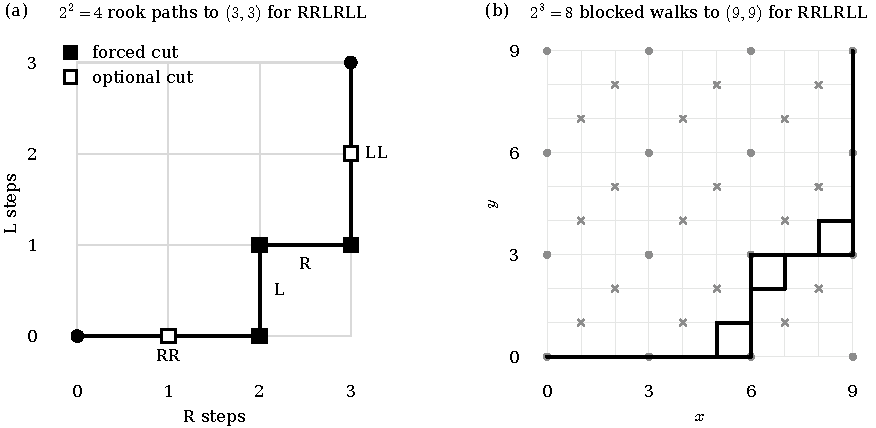
\includegraphics{figures/lattice}
\caption{The 2 bijections for the word $\sR\sR\sL\sR\sL\sL$. (a) The rook path. A cut
is forced at each of the $3$ direction changes (filled) and optional between
equal letters (hollow), so the word comes from $2^2=4$ rook paths to $(3,3)$.
(b) The union of the $2^3=8$ blocked walks to $(9,9)$ that give the word,
with 1 detour square for each direction change. Blocked points are marked
$\times$ and corners by dots.}
\label{fig:lattice}
\end{figure}

\begin{theorem}[$p=\tfrac23$ and rook paths]\label{thm:rook}
Let $r(a,b)$ count the rook paths from $(0,0)$ to $(a,b)$ with every move to the right or up. For
$p=\tfrac23$, $n_N(k)=r(k,N-k)$ for all $0\le k\le N$. Since the array of A035002 starts at $(1,1)$,
Kagey's $p=\tfrac23$ table read by rows is A035002 read by antidiagonals.
\end{theorem}

\begin{proof}
By definition each entry of A035002 is the sum of the entries to its left and above it, which is the
recursion for $r$ obtained by removing the last move. A rook path to $(a,b)$ with $a+b=N\ge1$ gives
a word $w$ with $a$ letters $\sR$ and $b$ letters $\sL$, one letter per unit of length, and a set of
cuts $i<N$ where one move ends and the next begins. A cut is forced where $w_i\ne w_{i+1}$ and
optional where $w_i=w_{i+1}$, and each choice of optional cuts gives exactly one rook path. Hence,
$r(a,b)=\sum_w2^{\rep(w)}$, which is $n_N(a)$ for $(\alpha,\beta)=(2,1)$ by
Proposition~\ref{prop:num}.
\end{proof}

\begin{theorem}[$p=\tfrac13$ and Mathar's blocked walks]\label{thm:mathar}
Call $(x,y)$ \emph{blocked} if $x\equiv y\equiv1$ or $x\equiv y\equiv2\pmod 3$, and let $M(a,b)$
count the walks from $(0,0)$ to $(3a,3b)$ with unit steps right and up that avoid blocked points.
For $p=\tfrac13$, $n_N(k)=M(k,N-k)$. The array $M$ is symmetric.
\end{theorem}

\begin{proof}
Work modulo $3$ and call a point with residue $(0,0)$ a \emph{corner}. Since $(1,1)$ and $(2,2)$ are
blocked, a right step from a corner is followed by another, to $(2,0)$, which we call state
$\mathsf A$, and an up step leads on to $(0,2)$, state $\mathsf B$. From $\mathsf A$ the walk steps
right to a corner, or it goes up, right and up to $\mathsf B$, and $\mathsf B$ behaves symmetrically. Leaving
$\mathsf A$ crosses one line $x\equiv0$ and no line $y\equiv0$, leaving $\mathsf B$ does the
reverse, and leaving a corner crosses neither. A walk to $(3a,3b)$ crosses $a$ lines $x\equiv0$ and
$b$ lines $y\equiv0$, so writing $\sR$ for each visit to $\mathsf A$ and $\sL$ for each visit
to $\mathsf B$ gives a word $w$ with $a$ letters $\sR$ and $b$ letters $\sL$. Between $w_i$ and $w_{i+1}$
the walk passes through a corner if $w_i=w_{i+1}$, in 1 way, and through a corner or directly if
$w_i\ne w_{i+1}$, in 2 ways. The start and the end are forced. Hence $M(a,b)=\sum_w2^{\chg(w)}$,
which is $n_N(a)$ for $(\alpha,\beta)=(1,2)$ by Proposition~\ref{prop:num}. Swapping the letters
$\sR$ and $\sL$ keeps $\chg(w)$, so $M(a,b)=M(b,a)$.
\end{proof}

In Mathar's note~\cite{mathar2022} the ``squares'' of A348595 are lattice points. A direct count
of the walks gives its published terms (computer-checked, Section~\ref{sec:verify}). So A348595
lists the lower triangle of $M$, which is how that entry is ``related'' to the $p=\tfrac13$ table.


\begin{thebibliography}{99}\small\setlength{\baselineskip}{11pt}\setlength{\itemsep}{0pt}\setlength{\parsep}{0pt}

\bibitem{kagey131}
P.~Kagey, \emph{Problem 131}, Open Problem Collection,
\url{https://peterkagey.com/problems/131/} (accessed September 2026).

\bibitem{paperB}
A.~Pemmasani, \emph{The middle and the ends II. Vertex crossings in a symmetric Markov multinomial
model}, preprint, 2026.

\bibitem{paperC}
A.~Pemmasani, \emph{The middle and the ends III. Face selection for slowly switching Markov chains and
the planar persistent walk}, preprint, 2026.

\bibitem{paperD}
A.~Pemmasani, \emph{The middle and the ends IV. Endpoint crossings for random walks with memory},
preprint, 2026.

\bibitem{antal2004}
T.~Antal, M.~Droz and Z.~R\'acz, \emph{Probability distribution of magnetization in the
one-dimensional Ising model: effects of boundary conditions},
J.~Phys.~A: Math.~Gen.~\textbf{37} (2004), 1465--1478.
\url{https://arxiv.org/abs/cond-mat/0308442}.

\bibitem{billingsley1995}
P.~Billingsley, \emph{Probability and Measure}, 3rd ed., Wiley, New York, 1995.

\bibitem{cekanavicius2001}
V.~\v{C}ekanavi\v{c}ius and M.~Mikalauskas,
\emph{Local theorems for the Markov binomial distribution},
Lithuanian Math.~J.~\textbf{41} (2001), 219--231.
\url{https://doi.org/10.1023/A:1012802428342}.

\bibitem{cekanavicius2001ld}
V.~\v{C}ekanavi\v{c}ius and M.~Mikalauskas,
\emph{Large deviations for the Markov binomial distribution},
Lithuanian Math.~J.~\textbf{41} (2001), 307--318.
\url{https://doi.org/10.1023/A:1013840819221}.

\bibitem{cekanavicius2010}
V.~\v{C}ekanavi\v{c}ius and P.~Vellaisamy, \emph{Compound Poisson and signed
compound Poisson approximations to the Markov binomial law}, Bernoulli
\textbf{16} (2010), 1114--1136. \url{https://doi.org/10.3150/09-BEJ246}.

\bibitem{cekanavicius2024}
V.~\v{C}ekanavi\v{c}ius and G.~Liaudanskait\.{e}, \emph{Skellam compound
Poisson approximation to the sums of symmetric Markov dependent random
variables}, arXiv:2404.17389 (2024).

\bibitem{dantchev2022}
D.~Dantchev and J.~Rudnick, \emph{Exact expressions for the partition function of the
one-dimensional Ising model in the fixed-$M$ ensemble},
Phys.~Rev.~E \textbf{106} (2022), L042103.
\url{https://arxiv.org/abs/2207.01134}.

\bibitem{dekkingkong2011}
F.~M.~Dekking and D.~Kong, \emph{Multimodality of the Markov binomial distribution},
J.~Appl.~Probab.\ \textbf{48} (2011), 938--953.
\url{https://arxiv.org/abs/1102.3613}. Proposition numbers as in the arXiv version.

\bibitem{elliott1971}
D.~Elliott, \emph{Uniform asymptotic expansions of the Jacobi polynomials and an associated
function}, Math.\ Comp.\ \textbf{25} (1971), 309--315.

\bibitem{ghosh2012}
R.~K.~Ghosh, \emph{A note on the Lee--Yang circle theorem}, arXiv:1201.3169
(2012).

\bibitem{gillis1955}
J.~Gillis, \emph{Correlated random walk}, Proc.\ Cambridge Philos.\ Soc.\ \textbf{51} (1955),
639--651.

\bibitem{goldstein1951}
S.~Goldstein, \emph{On diffusion by discontinuous movements, and on the telegraph equation},
Quart.\ J.\ Mech.\ Appl.\ Math.\ \textbf{4} (1951), 129--156.

\bibitem{herrmann2010}
S.~Herrmann and P.~Vallois, \emph{From persistent random walk to the telegraph noise},
Stochastics and Dynamics \textbf{10} (2010), 161--196.
\url{https://arxiv.org/abs/0810.0650}.

\bibitem{jensen2013}
J.~L.~Jensen, \emph{On a saddlepoint approximation to the Markov binomial
distribution}, Braz.\ J.\ Probab.\ Stat.\ \textbf{27} (2013), 150--161.
\url{https://doi.org/10.1214/11-BJPS162}.

\bibitem{konno2009}
N.~Konno, \emph{Limit theorems and absorption problems for one-dimensional correlated random
walks}, Stochastic Models \textbf{25} (2009), 28--49.
\url{https://arxiv.org/abs/quant-ph/0310191}.

\bibitem{leeyang1952}
T.~D.~Lee and C.~N.~Yang, \emph{Statistical theory of equations of state and
phase transitions. II. Lattice gas and Ising model}, Phys.\ Rev.\ \textbf{87}
(1952), 410--419. \url{https://doi.org/10.1103/PhysRev.87.410}.

\bibitem{mathar2022}
R.~J.~Mathar, \emph{Walks of up and right steps in the square lattice with blocked squares}
(January 2022), \url{https://oeis.org/A348595/a348595.pdf}.

\bibitem{oeisA035002}
E.~Friedman, Sequence A035002, in: OEIS Foundation Inc., \emph{The On-Line Encyclopedia of Integer
Sequences}, \url{https://oeis.org/A035002}.

\bibitem{oeisA348595}
R.~J.~Mathar, Sequence A348595, in: OEIS (2022), \url{https://oeis.org/A348595}.

\bibitem{pitman1997}
J.~Pitman, \emph{Probabilistic bounds on the coefficients of polynomials with only real zeros},
J.~Combin.\ Theory Ser.~A \textbf{77} (1997), 279--303.

\bibitem{renshaw1981}
E.~Renshaw and R.~Henderson, \emph{The correlated random walk}, J.\ Appl.\ Probab.\ \textbf{18}
(1981), 403--414.
\url{https://www.jstor.org/stable/3213286}.

\bibitem{stepanyan2024}
V.~Stepanyan, A.~F.~Tzortzakakis, D.~Petrosyan and A.~E.~Allahverdyan,
\emph{Thermal transitions in a one-dimensional, finite-size Ising model},
J.~Stat.~Mech. (2024), 033202.
\url{https://doi.org/10.1088/1742-5468/ad2679}.

\bibitem{temme1990}
N.~M.~Temme, \emph{Polynomial asymptotic estimates of Gegenbauer, Laguerre, and Jacobi
polynomials}, in: R.~Wong (ed.), \emph{Asymptotic and Computational Analysis}, Lecture Notes in
Pure and Appl.\ Math.\ \textbf{124}, Dekker, New York, 1990, 455--476.

\bibitem{dlmf}
NIST, \emph{Digital Library of Mathematical Functions}, Eqs.~10.25.2, 10.29.1,
10.29.2, 10.29.3, 10.32.3, 10.40.1, 18.7.21 and~18.11.5,
\url{https://dlmf.nist.gov/10.25.E2}, \url{https://dlmf.nist.gov/10.29},
\url{https://dlmf.nist.gov/10.32.E3}, \url{https://dlmf.nist.gov/10.40.E1},
\url{https://dlmf.nist.gov/18.7.E21}, \url{https://dlmf.nist.gov/18.11.E5}.

\end{thebibliography}

\end{document}
